\documentclass[11pt]{scrreport}

%von mir
\usepackage{setspace}
\usepackage[english]{babel}
%\usepackage[pdffitwindow=true, pdftex]{hyperref}
\usepackage[colorlinks=true,
pdffitwindow=true, 
pdftex,
linkcolor=black,
citecolor=black,
filecolor=black,
pagecolor=black,
urlcolor=black,
bookmarks=true,
bookmarksopen=true,
bookmarksopenlevel=3,
plainpages=false,
pdfpagelabels=true]{hyperref}
%von Mathes
\usepackage[margin=10pt, font=small, labelfont=bf, parskip=100pt]{caption}[2020/08/23] %von mir und Mathes
\captionsetup[figure]{justification=centering,labelfont=bf}

\usepackage[utf8]{inputenc} 	% ä,ö,ü,...
\usepackage[T1]{fontenc}
\usepackage{helvet}
\renewcommand{\familydefault}{\sfdefault}

\usepackage[
	inner=2cm,
	top=2cm,
	outer=2cm,
	bottom=2cm,
	headheight=40pt,
	marginparwidth=3cm
]{geometry}

\usepackage{graphicx}
\usepackage{xcolor}
% FHWS Farben
\definecolor{fhws-orange}{cmyk}{0,0.53,1,0}
\definecolor{fhws-green}{cmyk}{0.41,0,0.78,0}
\definecolor{fhws-gray-80}{gray}{0.2}
\definecolor{fhws-gray-60}{gray}{0.4}
\definecolor{fhws-gray-40}{gray}{0.6}
\definecolor{fhws-gray-20}{gray}{0.8}

\usepackage{booktabs} 	%	Tabellen schöner setzen	% \toprule, \midrule, \bottomrule

\usepackage{tikz}

\usetikzlibrary{arrows}
\usetikzlibrary{arrows.meta}
\usetikzlibrary{positioning}
\usetikzlibrary{shapes.geometric}



\usepackage{xspace}
\newcommand{\cpp}{\mbox{C$++$}\xspace}
\newcommand{\zB}{\mbox{z.\,B.}\xspace}
\newcommand{\dahe}{\mbox{d.\,h.}\xspace}
\newcommand{\ua}{\mbox{u.\,a.}\xspace}
\newcommand{\bzw}{\mbox{bzw.}\xspace}
\newcommand{\engl}{\mbox{engl.}\xspace}
\newcommand{\ggf}{\mbox{ggf.}\xspace}
\newcommand{\etc}{\mbox{etc.}\xspace}
\newcommand{\evtl}{\mbox{evtl.}\xspace}
\newcommand{\usw}{\mbox{usw.}\xspace}
\newcommand{\vs}{\mbox{vs.}\xspace}
\newcommand{\vgl}{\mbox{vgl.}\xspace}



\usepackage{marginnote}
\usepackage{menukeys}



%%% semantisches Markup
\newcommand{\begriff}[1]{\textcolor{fhws-orange}{\emph{\textbf{#1}}}}
\newcommand{\code}[1]{\texttt{#1}}
\newcommand{\todo}[1]{\textcolor{red}{#1}}
\newcommand{\datei}[1]{\textbf{#1}}
\newcommand{\name}[1]{\textsc{#1}}
\newenvironment{zitat}{\begin{itshape}\begin{center}}{\end{center}\end{itshape}}

%Code einfügen mit style=customc
\usepackage{listings}
\lstdefinestyle{customc}{
  belowcaptionskip=1\baselineskip,
  breaklines=true,
  frame=L,
  xleftmargin=\parindent,
  language=C,
  showstringspaces=false,
  basicstyle=\footnotesize\ttfamily,
  keywordstyle=\bfseries\color{green!40!black},
  commentstyle=\itshape\color{purple!40!black},
  identifierstyle=\color{blue},
  stringstyle=\color{orange},
}

\usepackage[backend=biber, style=apa]{biblatex}
%\addbibresource{export.bib}
\addbibresource{LiteraturVeraendert.bib}

\usepackage{acronym}

\renewcommand{\lstlistlistingname}{Quellcodeverzeichnis}

%fuer Seitenzahl im Hauptteil Seite x von y
%\usepackage{blindtext}
\usepackage[automark,autooneside=false,headsepline, footsepline]{scrlayer-scrpage}
\usepackage{lastpage} 
\usepackage{csquotes}
%\clearpairofpagestyles
%\ihead{\leftmark}
%\ohead{}

\ihead{\headmark}
\chead{}
\automark{chapter}
%\newcommand{\solutionsheet}{%
%  \clearpairofpagestyles
%  \ofoot*[{Seite \thepage\ von 26}]{Seite \thepage\ von 26}
%
%}

  

\lstset{
	language={},                % {} für normalen Klartext
	backgroundcolor=\color{white},
	linewidth=\linewidth,       % Zeilenbreite
	breaklines=true,             % Zeileumbruch
	breakatwhitespace=true, %Umbruch an Leerzeichen
%	caption = test listing       % Überschrift 
}


\begin{document}
		%DECKBLATT
\begin{titlepage}

  \title{ \centerline{
\includegraphics[scale=.6,]{Bilder/iuLogo.png}} 
    {\Large
      Computer Science\\
      written assignment\\
    }
     \vspace{45pt}
      Python as a Parser\\*[2ex] 

  }
	\author{\begin{tabular}{ll}
          	Author: & Xaver Gruber \\ Matriculation Number: & 42304184 \\
            Tutor: & Dr. Cosmina Croitoru \\
            Course Name: & Programming with Python \\
            Course Code: & DLMDSPWP01 \\
            Date: & \today \\
          \end{tabular}}

  \date{}

  \maketitle
\end{titlepage}

	\onehalfspacing
	%INHALTSVERZEICHNIS
		\tableofcontents
	\chapter*{Sperrvermerk}
		Die vorliegende Bachelorarbeit mit dem Titel \glqq Entwicklung und Optimierung einer Software-in-the-Loop-Teststrategie für elektrische Antriebsfunktionen\grqq{} 
enthält schützenswerte Informationen der ZF Friedrichshafen AG. Die Veröffentlichung, Vervielfältigung -auch in schriftlicher Form-, Weitergabe -auch auszugsweise- 
sowie das Einstellen dieser Abschlussarbeit in eine Hochschulbibliothek oder öffentlich zugängliche Bibliothek sowie jede weitere öffentliche 
Zugänglichmachung sind vor Ablauf der angegebenen Sperrfrist ohne vorherige schriftliche Zustimmung der ZF Friedrichshafen AG nicht gestattet. Ausgenommen 
von diesem Zustimmungserfordernis ist die Verwendung, die aufgrund der jeweils anwendbaren Prüfungs- oder Studienordnung 
zwingend erforderlich ist.\\
Die Sperrfrist gilt mit Abgabe der Abschlussarbeit an der Hochschule 3 Jahre.\\*[4ex]
Schweinfurt, 30.04.22
		
	\chapter*{Abkürzungsverzeichnis}
		\begin{acronym}[EuGH]

% \acro{eugh}[EuGH]{Europäischer Gerichtshof}

% \acro{eu}[EU]{Europäische Union} 
\acro{tpt}[TPT]{Time Partition Testing} 
\acro{sil}[SiL]{Software-in-the-Loop} 
\acro{mil}[MiL]{Model-in-the-Loop} 
\acro{pil}[PiL]{Processor-in-the-Loop} 
\acro{hil}[HiL]{Hardware-in-the-Loop} 

\acro{zf}[ZF]{ZF Friedrichshafen AG}
\acro{sut}[SUT]{System under Test}
\acro{api}[API]{Application Program Interface}
\acro{xml}[XML]{Extensible Markup Language}
\acro{exe}[exe]{executable}
\acro{api}[API]{Application Programming Interface}





\end{acronym}
		
		
	\addchap{Abstract}
		This bachelor thesis is about two topics as Software-in-the-Loop test strategy. One topic is
Interface Testing; the other one is Equivalence Classes. Both topics are worked out within TPT, which
is a software for testing embedded systems by the company PikeTec. Steps for Interface Testing include
analyzing the existing Interface Test, modelling a C source and automatically generating test cases using TPT.
A concept for Equivalence Classes is pointed out, which is about validating existing Software-in-the-Loop tests
and self-tests checking if the defined Equivalence Classes are reached. It is explained that defining the latter is a way of creating
a database that can be used for further tests.
	\addchap{Kurzfassung}
		%Diese Arbeit handelt von einer Software-in-the-Loop Teststrategie für elektrische Antriebsfunktionen.
%TPT ist ein Programm, das ursprünglich bei der Daimler AG entwickelt wurde, um eingebettete Systeme zu testen.
Es werden zwei Themen als Software-in-the-Loop Teststrategie bearbeitet, nämlich ein Schnittstellentest und ein Äquivalenzklassentest.
Beide Themen werden mit TPT erarbeitet. TPT ist ein Programm der Firma PikeTec zum Testen von eingebetteten Systemen.
Die Arbeitspakete für den Schnittstellentest sind einen bestehenden Schnittstellentest zu analysieren, 
eine C Datei nachzustellen und Testfälle automatisiert in TPT generieren lassen.
% Ein bestehender Schnittstellentest wird analysiert. Eine C Datei wird für den Schnittstellentest in TPT 
% nachgestellt. Die Testfälle werden automtatisiert in TPT generiert.
Für den Äquivalenzklassentest wird ein Konzept erarbeitet, wie diese eingesetzt werden können.
Es geht zum Einen darum, Äquivalenzklassen zu nutzen, um bestehende Software-in-the-Loop Tests zu überprüfen.
Zum Anderen geht es um eine Selbstüberprüfung der Äquivalenzklassen, ob die definierten Äquivalenzklassen alle erreichbar sind.
Es wird auch aufgezeigt, dass durch das Definieren von Äquivalenzklassen eine gewisse Datenbank für Tests entsteht und 
diese auch für weitere Tests eingesetzt werden kann.

% dass dadurch für Signale systematisch Werte festgelegt werden und somit eine Datenbasis angelegt wird,
% die auch für weitere Testfälle eingesetzt werden können.

% um eine Datenbasis zu erreichen, indem Werte definiert sind, die später auch für andere Tests eingesetzt werden
% können.

	% Test footcite \footcite{TPT}
	%Test cite \cite[Vgl.][S.223]{TPT}
	% Zitat parencite1 \parencite{TPT}. \\
% %Zitat 2 \cite{Test}. \\
% textcite 3 \textcite{TPT}. \\
% footcite 4 \footcite{TPT}. \\
% footfullcite 5 \footfullcite{TPT}. \\
% %Das zweite Beispiel \footcite[Vgl.][S.223]{hacker}.
% %Das dritte Beispiel \footcite[Vgl.][S.223]{hacker}.

	
	\chapter{Einleitung}
	\newcounter{generell}
	\setcounter{generell}{\value{page}}
	\pagenumbering{arabic}
	
		\section{Vorstellung der ZF}
			


\ac{zf} ist ein Technologiekonzern mit rund 153.500 Mitarbeitern (Stand 2020) weltweit in den Bereichen Mobilität
und Industrietechnik. ZF übernahm zuletzt WABCO und konnte dadurch ihre Kompetenz im Bereich von Technologien
für schwere Nutzfahrzeuge, Busse und Trailer steigern. ZF gibt jährlich sieben Prozent des Umsatzes (Stand 2020) in 
Forschung und Entwicklung aus. ZF will die Veränderungen in der Mobilitätsbranche 
% spürt Veränderungen in der Mobilitätsbranche und will die Zukunft 
mit der
Strategie \glqq Next Generation Mobility\grqq{} vorantreiben. Das Ziel der Strategie ist eine einfache, saubere
Mobilität, die automatisiert, komfortabel und bezahlbar ist. Sie soll für jedermann und überall erreichbar sein.
Für die Bachelorarbeit bin ich in der Abteilung Softwareentwicklung elektrische
Antriebsfunktionen tätig \cite[vgl.][]{zf}.

% Quelle: https://www.zf.com/mobile/de/company/company.html    (in Literaturrecherche gespeichert)
% Abruf 28.01.22 um 14:22 Uhr
		\section{Beschreibung des Themas}
			Antriebsfunktionen elektrischer Maschinen sind als Software geschrieben, laufen auf einer 
Hardware und übernehmen die Steuerung der Maschine. Das macht ein eingebettetes System aus.
Ein eingebettetes System ist in der Regel ein in-the-Loop System. In einem in-the-Loop System bilden Ausgänge des Systems
eine Rückkopplung zu den Eingängen. Dies muss auch beim Testen berücksichtigt werden.
Software-in-the-Loop Test bedeutet, dass die Software als in-the-Loop System getestet wird, wobei die Hardware
simuliert wird. Bei Hardware-in-the-Loop hingegen ist die Hardware vorhanden und die Software wird, während
es auf der Hardware ausgeführt wird, getestet.
Mit SIL wird eine Möglichkeiten geschaffen Software ohne Hardware zu testen. Damit können Kosten von Hardware eingespart werden.
%SIL ist in der Entwicklung bedeutend, da es keine Hardware zum Testen benötigt. Damit können Kosten von Hardware eingespart werden.
Des Weiteren kann dadurch auch in den frühen Phasen der Entwicklung getestet werden \parencite[S. 1 f.]{silest}\parencite[]{hilwikipedia}. Es ist wichtig Fehler schnell zu beheben,
denn je länger ein Fehler unentdeckt bleibt, umso teurer wird dieser Fehler \parencite[]{fehler}.

Diese Arbeit handelt davon TPT als Programm (siehe Abschnitt 1.4) einzusetzen, um einen Schnittstellentest zu überführen (siehe Kapitel 5) und ein
neues Testkonzept mit Äquivalenzklassen (siehe Kapitel 6) zu erarbeiten.




% Beschreibung software-in-the-Loop für elektrische Ant
% in the Loop allgemein -> zur Steuerung elektrischer Maschinen\\
% software-in-the-Loop -> Virtualisierung der Hardware\\
% Schnittstellentest, Äquivalenzklassentest

% Was ist software-in-the-loop? Wichtigkeit von Testen allgemein
% SIL; HIL, MIL
% Was bedeutet in the loop? Warum die Namensgebung?
% Seit wann gibt es SIL, warum wurde es eingeführt? Nutzen?

% Einordnung der Bachelorarbeit, welchen Bereich umfasst die Bachelorarbeit
% Interesse wecken, 
% genaue Beschreibung des Themas
% Ziele der Bachelorarbeit
% Nutzen der Bachelorarbeit für ZF, die Wissenschaft
		\section{Einordnung der Arbeit}
			% % Einordnung in SIL, MIL, HIL, was ist Testen allgemein?
% % Weiter in black box, dynamisch und funktional ( ist die Einordnung der Äquivalenzklassen)
% % Grob das ganze Umfeld erklären und Sachen wie black box testing näher erklären
% %in the Loop erklären
% Antriebsfunktionen elektrischer Maschinen sind als Software geschrieben, laufen auf einer 
% Hardware und übernehmen die Steuerung der Maschine. Das macht ein eingebettetes System aus.
 % % zu testen. Es 
% % Die Steuerung elektrischer Maschinen ist ein eingebettetes System, wobei der Motor von einem
% % Mikrocontroller gesteuert wird.
% Ein eingebettetes System ist in der Regel ein in-the-Loop System. In einem in-the-Loop System bilden Ausgänge des Systems
% eine Rückkopplung zu den Eingängen. Dies muss auch beim Testen berücksichtigt werden.

% Software-in-the-Loop bedeutet, dass die Software als in the Loop System getestet wird, wobei die Hardware
% simuliert wird. Bei Hardware-in-the-Loop hingegen ist die Hardware vorhanden und die Software wird, während
% es auf der Hardware ausgeführt wird, getestet.
% SIL ist in der Entwicklung bedeutend, da es keine Hardware zum Testen benötigt und schon in den 
% frühen Phasen der Entwicklung getestet werden kann\cite[S.1 f.]{silest}. Je länger ein Fehler unentdeckt bleibt und nicht
% behoben wird, umso teurer wird dieser Fehler.

% Diese Arbeit handelt davon TPT als Programm einzusetzen, um einen Schnittstellentest zu überführen und ein
% neues Testkonzept mit Äquivalenzklassen zu erarbeiten.
% Diese Arbeit handelt von der Entwicklug eines Konzepts für Äquivalenzklassen und Überführung eines 
% Schnittstellentests. Beides in TPT.
In der Abteilung Softwareentwicklung elektrische Antriebsfunktion bei ZF, in der ich für die Bachelorarbeit tätig bin,
wird nach dem V-Modell entwickelt (siehe Abbildung 1.1).\par
\begin{figure}[h]
\centering
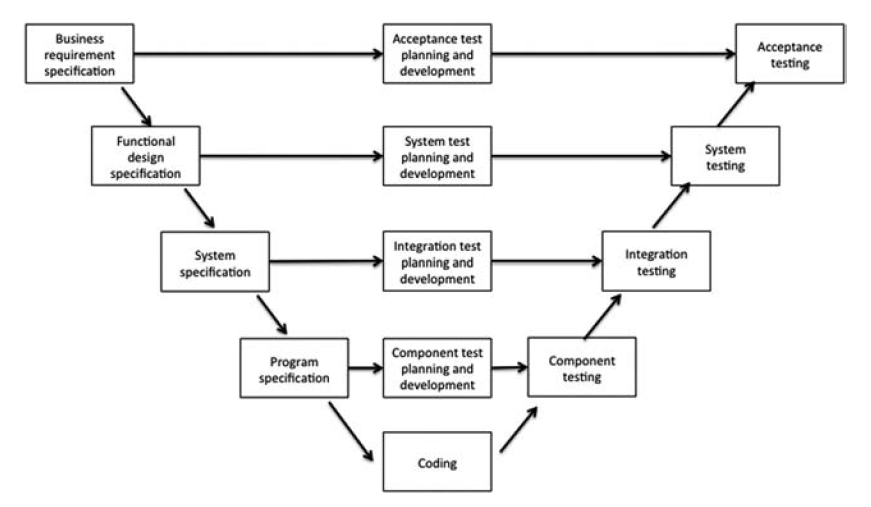
\includegraphics[scale=1.2,]{Bilder/VModell.png}
\caption{V-Modell \cite[S. 68]{agiletesting}}\label{fig:VModell}
\end{figure}
Ein Merkmal des V-Modells ist, dass jede Stufe der Entwicklung einen dazugehörigen Test besitzt.
Die folgenden Testebenen beschreiben die einzelnen Teststufen \cite[vgl.][S. 41 f., S. 51]{integration}:
\begin{description}
\item[Komponententest] Es wird eine Komponente isoliert von der Software - funktional und strukturell - getestet. % \cite[vgl.][S. 41]{integration}
\item[Integrationstest] Es ist ein Test, der das Zusammenspiel bereits getesteter Komponenten überprüft. %  \cite[vgl.][S. 51]{integration}. 
\item[Systemtest] Es wird die Funktionsfähigkeit des ganzen Systems getestet. Dazu zählen auch Performanz-, Stress und Robustheitstests.
\item[Abnahmetest] Mit diesem Test wird überprüft, ob die Erwartungen der Anwender erfüllt werden. Der Test soll
unter realen Einsatzbedingungen stattfinden.
\end{description}
%Im Komponententest wird eine Komponente isoliert vom Rest der Software getestet. %\cite[S.41]{integration}.
%Die Komponente wird funktional und strukturell getestet \cite[vgl.][S. 41]{integration}.
% Das ist der erste Test nach der Implementation.
% Der Komponententest zeichnet sich aus, dass einzelne elementare Programmbausteine isoliert getestet werden.
% Im Modultest bzw. Komponententest (unit test) werden einzelne elementare Programmbausteine
% isoliert getestet, oft vom jeweiligen Entwickler selbst. Die Bausteine bzw. Testobjekte
% können dabei auch zusammengesetzt sein. Der Tester hat in der Regel Zugang zum Quellcode,
% sodass in dieser Teststufe sehr entwicklungsnah gearbeitet wird und es sind somit
% sowohl Black-Box- als auch White-Box-Verfahren anwendbar.
%Der Integrationstest ist ein Test, der das Zusammenspiel bereits getesteter Komponenten überprüft \cite[vgl.][S. 51]{integration}. 
%Fehler in den Schnittstellen sollen hier aufgedeckt werden.
% Wichtig:
% Es gibt verschiedene Integrationsstufen, die der Reihe nach getestet werden.(hier Integrationsstufen aufzählen).
%Hier Erklärung Integrationstest und Erklärung Komponententest einfügen.
%Jede Stufe der Entwicklung besitzt einen dazugehörigen Test.
Der Schnittstellentest, in dem die Signalverbindungen zwischen Komponenten überprüft werden, ist ein Teil des 
Integrationstests \cite[vgl.][S. 51, S. 217]{integration}.
Der Äquivalenzklassentest ist als funktionaler Test im Komponententest wiederzufinden \cite[vgl.][S. 41 f.]{integration}\cite[vgl.][S. 114 ff.]{equiinformatic}.

Wie der Äquivalenzklassentest einzuordnen ist, wird in Abbildung 1.2 deutlich.
Dieses Diagramm ist nicht vollständig, sondern soll nur als Einordnung dienen.
Eine Art der Analyse in der Software ist eine dynamische Analyse, eine weitere ist die statische Analyse.
In der dynamischen Analyse
wird der Code ausgeführt, in der statischen hingegen nicht. Eine Art der dynamischen Analyse ist funktional, eine weitere Art ist strukturell.
In der funktionalen Analyse wird das System als Kasten betrachtet, sprich Informationen über den Programmcode sowie
der inneren Struktur sind nicht von Bedeutung. Deshalb wird es auch als Blackbox-Testverfahren bezeichnet.
In der strukturellen Analyse hingegen wird der innere Ablauf im Testobjekt analysiert. Der Blickwinkel wandert
in das System. Es wird auch Whitebox-Testverfahren genannt.
Ein funktionaler Test ist der Äquivalenzklassentest. 
Ein weiterer ist die Grenzwertanalyse \cite[vgl.][S. 114 ff.]{equiinformatic}\cite[vgl.][]{dynamischeanalyse1}\cite[vgl.][]{dynamischeanalyse2}.
Die Grenzwertanalyse eignet sich hervorragend, um sie mit anderen Tests wie dem Äquivalenzklassentest 
zu kombinieren \cite[vgl.][S. 36]{integration}.\par
\begin{figure}[h]
\centering
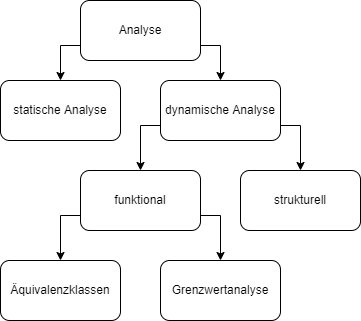
\includegraphics[scale=0.9,]{Bilder/Einordnung.drawio.png}
\caption{Einordnung der Äquivalenzklassen \cite[vgl.][]{dynamischeanalyse1}\cite[vgl.][]{dynamischeanalyse2}\cite[vgl.][S. 114 ff.]{equiinformatic}}
\end{figure}



% Schnittstellentest, Teil des Integrationstests.
% Äquivalenzklassentest ist Komponententest nach Abbildung V Modell.
% Analysearten Äquivalenzklassentest:
% dynamisch, statisch. Bla bla erklären nach Abbildung (Einordnung der Äquivalenzklassen)


% Verifikation und Validation umfasst 30-50% des Entwicklunsgaufwands
% Oftmals erst möglich, wenn Hardware vorhanden ist
% Keine Hardware: geringe Parallelisierbarkeit Entwicklung von Hard und Software
% Abhilfe: SIL
% Verifikation erschwert durch minimale Software-Schnittstellen
% Ausgänge von embedded systems Rückkopplung auf eigene Eingänge
% Software kann nicht losgelöst von technischem Umfeld getestet werden
% Untersuchung des Regelkreises notwendig(SIL ist Closed Loop, nicht open loop)
% Besonders wichtig: Test der Auswirkungen von Sensor und Aktuator Fehlverhalten
% SIL: Nachbildung des umgebenden technischen Systems als eine realistische und ausführbare Software-Simulation
% Vorteile: kostengünstiger, umfassender, wiederholbar, automatisierbar, rückverfolgbar






% SIL wird eingesetzt, da es viel 
% Besonders wichtig ist das Fehlverhalten von Sensoren und Aktuatoren zu testen.
% Test der Auswirkungen von Sensor und Aktuator Fehlverhalten


% \begin{figure}[h]
% \centering
% 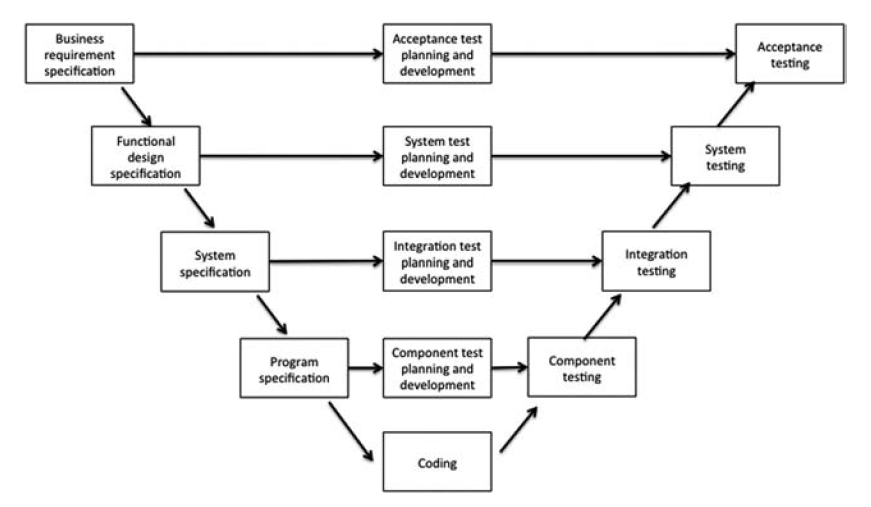
\includegraphics[scale=1.2,]{Bilder/VModell.png}
% \caption{V-Modell}
% \end{figure}
% \begin{figure}[h]
% \centering
% 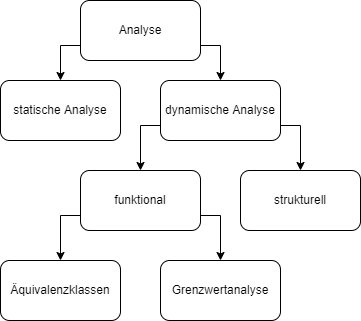
\includegraphics[scale=0.9,]{Bilder/Einordnung.drawio.png}
% \caption{Einordnung der Äquivalenzklassen}
% \end{figure}



% Quelle über dynamischer Test,black box (Äquivalenzklassen): Basiswissen\_Softwaretest...pdf\\

% % Von Y:\Bachelor\Bachelorarbeit\Basiswissen_Softwaretest_Aus-_und_Weiterbildung_zu..._----_(Pg_131--193).pdf

% % Bis Seite 148 geht es um Blackbox-Verfahren

% % Ziel des Testens: Nachweis der Erfüllung der festgelegten Anforderungen

% Dynamischer Test -> Blackbox -> Äquivalenzklassen\\

% Systematische Erstellung von Testfällen:
% % Blackbox Verfahren und whitebox Verfahren
% % "Die vorausgesagten Ergebnisse (Ausgaben, Änderung von internen
% % Zuständen usw.) müssen vor der Ausführung der Testfälle feststehen
% % und dokumentiert werden."
% % (In Softcar, der setpoint wird berechnet durch die Eingangswerte
% % Danach wird überprüft, ob das Programm auf das gleiche Ergebnis wie der setpoint gekommen ist)

% "Bei den Blackbox-Verfahren wird das Testobjekt als schwarzer
% Kasten angesehen. Über den Programmtext und den inneren Aufbau
% sind keine Informationen notwendig."\\

% "Bei den Whitebox-Verfahren wird auch auf den Programmtext
% zurückgegriffen. Während der Ausführung der Testfälle wird der
% innere Ablauf im Testobjekt analysiert (der Point of Observation liegt
% innerhalb des Testobjekts)."\\

% Blackbox: spezifikationsbasiertes Testentwurfsverfahren\\

% Whitebox: strukturelles Testverfahren\\

% dynamischer vs statischer Test\\

% Diagramm zeichnen mit der Einordnung von den unterschiedlichen Testarten(dynamisch, statisch, black box etc.)


% % Trends in Software Testing

% % SILreliability
% % SILreliability Vergleich von sil und hil, Trend geht dazu, dass mehr Hardware Sachen mit Software gelöst werden, V Modell zeigt sil ist für module und auch Integrationstest, Vorteil von sil gegenüber Hil ist, dass mit sil kein corrupted data entstehen kann (unter 4. Results)

% % \begin{lstlisting}
% % Virtual platforms von Software-in-the-Loop_simulation_of_embedded_control_applications_based_on_Virtual_Platforms.pdf
% % \end{lstlisting}
% % Ist ein Trend zur embedded software Entwicklung

% % "Another advantage
% % of using virtual platforms in the early stage of the software
% % development is that they allow observing the behavior of the
% % entire system which leads to excellent debugging options
% % compared to the “black box”-like behavior of embedded
% % devices."


% % Another advantage
% % of using virtual platforms in the early stage of the software
% % development is that they allow observing the behavior of the
% % entire system which leads to excellent debugging options
% % compared to the “black box”-like behavior of embedded
% % devices.
		\newpage
		\section{TPT}
			%Quelle Dissertattion TPT\\
% Unter dem Titel \glqq Systematischer Test des kontinuierlichen Verhaltens von eingebetten Systemen\grqq{} wurde \ac{tpt} im Rahmen
% einer Dissertation von Eckard Lehmann bei der Daimler AG entwickelt. 
Eingebettete Systeme zeichnen sich aus, dass sie über kontinuierliche Größen,
etwa Sensoren, mit der Umgebung verbunden sind. \ac{tpt} wurde im Rahmen einer Dissertation von Eckard Lehmann bei der Daimler AG entwickelt, 
um das kontinuierliche Verhalten eingebetteter Systeme testen zu können. Die ersten Versionen gibt es schon im Jahre 2000.
Es wird jahrelang bei der Daimler AG in der Fahrzeugentwicklung benutzt und weiterentwickelt. Heutzutage besitzt \ac{tpt} die Firma PikeTec. 
Es werden eine Anbindung zu verschiedenen Programmen wie Autosar, Matlab, Labcar und Targetlink und verschiedene Testarten wie \ac{sil}, \ac{hil} \ac{mil},
\ac{pil} unterstützt. Das Programm ist von der Anforderungsanalyse über die Testfallerstellung bis zur Auswertung der Ergebnisse einsetzbar \cite[vgl.][]{piketecwebseite}\cite[vgl.][]{tptwikipedia}.
%Es besitzt einen Support zu verschiedenen Porgrammen wie Autosar, Matlab, Labcar, TargetLink etc
\ac{tpt} ist \cite[vgl.][S. 120]{tpt}:
\begin{itemize}
\item plattformunabhängig: Plattformen können ausgetauscht werden, ohne dass Testfälle neu geschrieben werden müssen
%dadurch können Platformen ausgetauscht werden, ohne dass die Testfälle neu geschrieben werden
\item echtzeitfähig: Echtzeitanforderungen eines eingebetteten Systems werden erfüllt
%\item echtzeitfähig: bei einem Echtzeitbetriebssystem soll die Testdurchführung Echtzeitanforderungen erfüllen
%Echtzeitanforderungen eines eingebetteten Systems werden erfüllt
\item reaktiv: beim Eintritt eines Systemzustands kann der Testfall darauf reagieren
\end{itemize}
Nun soll \ac{tpt} bei \ac{zf} in der Abteilung Softwareentwicklung elektrische Antriebsfunktionen eingeführt werden.
Es soll als einheitliche Testumgebung für \ac{sil} dienen und andere Tools wie Softcar, das ein \ac{zf} internes Tool ist, ablösen.



%Dadurch sollen Einschänkungen von Softcar(siehe Abschnitt XY) gelöst werden.



% Im Rahmen einer Dissertation von Eckard Lehmann wurde TPT bei Daimler entwickelt 
 % Das Ziel von TPT ist es, einen systematischen Ansatz für den Test eingebetteter Systeme zu erarbeiten.
% verbunden sind und dadurch mit 
% von realen Umgebungen 
% beeinflusst werden
 % Eingebettete Systeme beeinflussen reale umgebungen und kommunizieren mit dieser Umgebung in der Regel über 
% kontinuierliche Größen. Das Ziel der Arbeit war, dass ein spezialisierter systematischer Ansatz gegeben ist um eingebettete Systeme zu testen.
% Mit TPT kann man den ganzen Ablauf eines Tests von der Testfallerstellung bis zur Anforderungsanalyse alles abdecken.
% Die ersten Versionen gab es schon 2000. TPT wurde jahrelang von Daimler für ihre eigene Fahrzeugentwicklung benutzt. Heutzutage besitzt piketec 
% TPT und entwickelt es weiter. (Piketec Webseite(https://piketec.com/de/tpt/))
% TPT ist:
% \begin{itemize}
% \item plattformunabhängig

% \item echtzeitfähig

% \item reaktiv
% \end{itemize}

% 20 Jahre nach der ersten Version wird TPT bei ZF eingeführt werden.
% Es soll als einheitliche Testumgebung für \ac{sil} dienen und andere Tools wie Softcar, was ein ZF interenes Tool ist, ablösen.
% Dadurch sollen Einschänkungen von Softcar(siehe Abschnitt XY) gelöst werden.
% \ac{tpt} heißt auf Deutsch übersetzt
% TPT steht für? Englisch: Time Partition Testing  Deutsch:\\

% Was ist TPT?\\
% TPT wurde von Eckard Lehmann in seiner Dissertation bei Daimler entwickelt (von 2004)
% Daimler hat jahrelang selbst TPT weiterentwickelt. Heutzutage besitzt piketec TPT und entwickelt es weiter.
% Piketec Webseite(https://piketec.com/de/tpt/)
% "
% TPT unterstützt alle Testaktivitäten von der Testfallerstellung/-Generierung, der Testausführung, der Testauswertung und dem Testreporting, sowie dem Testmanagement und der Anforderungsanalyse."
% \\
% TPT besitzt auch großen Support zu verschiedenen Porgrammen wie Autosar, Matlab, Labcar, TargetLink etc (
 % "MiL Testing, SiL Testing, PiL Testing, HiL Testing, ECU Testing und Fahrzeugtests ausgeführt werden")
% \\
% Aus <https://piketec.com/de/tpt/> 

% TPT wurde von Daimler für ihre eigene Fahrzeigentwicklung ursprünglich entwickelt.


% Kurz erklären, was kann TPT alles?\\

% Warum wurde TPT entwickelt?\\
% TPT Ziel: Test von eingebetteten Systemen
% Zu dieser Zeit noch keine spezialisierte systematische Ansätze eingebettete Systeme zu testen
% Schwierigkeit embedded systems beeinflussen reale Umgebungen und kommunizieren mit dieser Umgebung in der Regel über kontinuierliche Größen(Sensoren)

% % (
% % Black-box, Zustände werden als Eingänge aufgefasst, sodass bei der Testdurchführung ein bestimmter Zustand eintritt, der gestestet werden soll

% % "Hat ein System beispielsweise drei Be-
% % triebsmodi, in denen es sich jeweils unterschiedlich verhÄalt, so wird fÄur einen
% % Testfall beschrieben, in welchem Betriebsmodus dieser Testfall durchzufÄuhren
% % ist."
% % )

% TPT ist (Kapitel 6)\\
% Plattformunabhängig:\\

% Echtzeitfähig:\\

% Reaktiv:\\


% Warum wird TPT bei ZF eingeführt?\\
% Eine einheitliche Testumgebung für SIL, Ablösen von Softcar und anderen Testumgebungen(Tessy)
% Eine Testumgebung, die alle Tests von Softcar und Tessy durchführen kann und Probleme von Softcar behebt(wie zum Beispiel manuelle Debug Ausgaben in Softcar), 
% für TPT müssen nicht Debug Ausgaben manuell geschrieben werden


% %Quelle Dissertattion TPT\\
		
		\section{Ziele}
			Ein Ziel der Arbeit ist einen bestehenden Schnittstellentest in TPT zu überführen und zu optimieren.
TPT soll als einheitliche Testumgebung eingeführt werden. Dabei werden bestehende Tests, so auch der Schnittstellentest,
in TPT überführt. Der Schnittstellentest hat Potenziale in der Laufzeit (siehe Kapitel 3), was opimiert werden soll.
Ein zweites Ziel ist ein Konzept für den Äquivalenzklassentest in TPT zu erarbeiten (siehe Kapitel 6). 


% Optimieren des Quicktests, Einführung in TPT\\
% Konzept  und Möglichkeiten(Testszenarien) für Äquivalenzklassentest

% KEINE ZIELE?????\\
% Ein Ziel ist die Umsetzung.\\
% Unterschiede von state of the art zu status quo erkennen.\\
% Umsetzung möglichst nahe an state of the art.\\
% Quicktest optimieren, Äquivalenzklassentest einführen.
	
			
			
	%\chapter{Methoden}
		% \section{Stand der Technik}
				% \subsection{in der Wissenschaft}
			% Quelle über dynamischer Test,black box (Äquivalenzklassen): Basiswissen\_Softwaretest...pdf\\

% Von Y:\Bachelor\Bachelorarbeit\Basiswissen_Softwaretest_Aus-_und_Weiterbildung_zu..._----_(Pg_131--193).pdf

% Bis Seite 148 geht es um Blackbox-Verfahren

% Ziel des Testens: Nachweis der Erfüllung der festgelegten Anforderungen

Dynamischer Test -> Blackbox -> Äquivalenzklassen\\

Systematische Erstellung von Testfällen:
% Blackbox Verfahren und whitebox Verfahren
% "Die vorausgesagten Ergebnisse (Ausgaben, Änderung von internen
% Zuständen usw.) müssen vor der Ausführung der Testfälle feststehen
% und dokumentiert werden."
% (In Softcar, der setpoint wird berechnet durch die Eingangswerte
% Danach wird überprüft, ob das Programm auf das gleiche Ergebnis wie der setpoint gekommen ist)

"Bei den Blackbox-Verfahren wird das Testobjekt als schwarzer
Kasten angesehen. Über den Programmtext und den inneren Aufbau
sind keine Informationen notwendig."\\

"Bei den Whitebox-Verfahren wird auch auf den Programmtext
zurückgegriffen. Während der Ausführung der Testfälle wird der
innere Ablauf im Testobjekt analysiert (der Point of Observation liegt
innerhalb des Testobjekts)."\\

Blackbox: spezifikationsbasiertes Testentwurfsverfahren\\

Whitebox: strukturelles Testverfahren\\

dynamischer vs statischer Test\\

Diagramm zeichnen mit der Einordnung von den unterschiedlichen Testarten(dynamisch, statisch, black box etc.)


% Trends in Software Testing

% SILreliability
% SILreliability Vergleich von sil und hil, Trend geht dazu, dass mehr Hardware Sachen mit Software gelöst werden, V Modell zeigt sil ist für module und auch Integrationstest, Vorteil von sil gegenüber Hil ist, dass mit sil kein corrupted data entstehen kann (unter 4. Results)

% \begin{lstlisting}
% Virtual platforms von Software-in-the-Loop_simulation_of_embedded_control_applications_based_on_Virtual_Platforms.pdf
% \end{lstlisting}
% Ist ein Trend zur embedded software Entwicklung

% "Another advantage
% of using virtual platforms in the early stage of the software
% development is that they allow observing the behavior of the
% entire system which leads to excellent debugging options
% compared to the “black box”-like behavior of embedded
% devices."


% Another advantage
% of using virtual platforms in the early stage of the software
% development is that they allow observing the behavior of the
% entire system which leads to excellent debugging options
% compared to the “black box”-like behavior of embedded
% devices.
				% \subsection{bei ZF}
			% Softcar - Quicktest, SIL Tests\\
Tessy - Requirements\\
Polyspace - statische Analyse von C Code\\
		% \section{TPT als Programm}
			% In Abbildung 2.5 ist ein Überblick zu sehen, welche Schritte nötig sind, um TPT für einen Test einzurichten \cite[vgl.][S. 39]{userguide}. 
%Im Folgenden ist zu sehen, welche Schritte benötigt werden, um TPT für einen Test einzurichten:
\begin{figure}[!h]
    \centering


  \begin{tikzpicture}%[every node/.style={rectangle,draw,text width=14em,align=center}]
    [
      % Stil für Ein- und Ausgabe
      io/.style={trapezium, trapezium left angle=70, trapezium right angle=110, fill=magenta!10, draw=magenta},
      % Stil für Operationen
      op/.style={rectangle, fill=orange!10, draw=orange},
      op4/.style={rectangle, fill=green!20, draw=green},
			op2/.style={rectangle, fill=green!20, draw=green, minimum height=2cm, minimum width=38mm},
			op3/.style={rectangle, fill=orange!10, draw=orange, minimum height=2cm, minimum width=38mm},
      % Stil für Entscheidungen
      cn/.style={diamond, aspect=2, inner sep=1pt, fill=red!10, draw=red, minimum width=20mm, minimum height=14mm},
      cn2/.style={diamond, aspect=2, inner sep=1pt, fill=blue!20, draw=blue, minimum width=20mm, minimum height=14mm},% Distanz zwischen den Knoten
      node distance=4mm]
    % Knoten
    %\node[op4] (class) {GSIL Projekt als Ausgang};
    
    \node[op4] (init) {C-Plattform Konfiguration};
    \node[op4, below=of init] (list) {Analysieren der Dateien};
    %\node[op, below=of list] (firstitem) {select first item in list};
%    \node[cn2, below=of list] (cond1) {};
    \node[op4, below=of list] (compile) {Generieren des TPT Testrahmens und Kompilieren};
    \node[op4, below=of compile] (depnewlist) {Testfallerstellung};
    \node[op4, below=of depnewlist] (execution) {\textit{Execution} Konfiguration};
    \node[op4, below=of execution] (final) {Testdurchführung};
%    \node[cn2, below=of depnewlist] (cond2) {};
    %\node[op, right=of cond2] (wrongdep) {select next item};
    %\node[op, below=of cond2] (makefiles) {search for item in dictionary to get makefiles};
    % \node[op4, below=of cond2] (initdep) {initialize object using item};
    % \node[op4, below=of initdep] (addobject) {add to object list};
    % \node[cn2, below=of addobject] (cond3) {\shortstack{last item from \\ dependency list?}};
    % \node[op4, right=of cond3] (wrongdep) {select next item};
    % \node[op4, below=of cond3] (findsubs) {object.findSubdirectories()};
    % \node[op4, below=of findsubs] (findfiles) {object.findFiles()};
    % \node[cn2, below=of findfiles] (cond4) {\shortstack{last item from\\ object list?}};
    % \node[op4, left=of cond4] (wrongobject) {select next item};
    % \node[op4, below=of cond4] (end) {Ende};
    
    \path[->]
		%(class) edge (init)
		(init) edge (list)
		(list) edge (compile)
		(compile) edge (depnewlist)
		(depnewlist) edge (execution)
		(execution) edge (final);
      % (finddep) edge (depnewlist)
      % (depnewlist) edge (cond2)
      % (cond2) edge (initdep)
      % (initdep) edge (addobject)
      % (addobject) edge (cond3)
      % (cond3) edge node[above=0.2cm] {No}(wrongdep)
      % (cond3) edge node[right=0.2cm] {Yes} (findsubs)
      % (findsubs) edge (findfiles)
			% (findfiles) edge (cond4)
      % (cond4) edge node[above=0.2cm] {No}(wrongobject)
      % (cond4) edge node[left=0.5cm] {Yes} (end);

    % \draw[->] 
      % (wrongdep) --  ++(2,0) |- (cond2)
      % (wrongobject) -- ++(-2,0) |- (cond1);
		% \draw[->] (cond2) -- node[below] {Nein} ++(2.9,0) -- (entscheid);
		% \draw[->] (cond4) -- node[below] {Nein} ++(4.0,0) -| (gescheitert2);
		% \draw[->] (cond3) -- node[below] {Nein} ++(-4.0,0) -| (gescheitert3);
      %(wrongdep) edge (cond1);
			% (cond1) edge node[right] {Ja} (cond2)
			% (cond2) edge node[below] {Ja} (gesetz2);
    
    % \node[cn, align=center, below=of begehren] (cond1) {okay\\Unterschriften?};
		% \node[cn, align=center, below=of cond1] (cond2) {Landtag nimmt\\Gesetzentwurf an?};
		% \node[op3, align=center, right=of cond1] (gescheitert) {Volksbegehren\\gescheitert};
		% \node[op, align=center, right=of cond2] (entscheid) {Volksentscheid};
		% \node[io, below=of entscheid] (abstimmung) {Stimmen Sie ab!};
		% \node[cn, align=center, below=of abstimmung] (cond3) {Mehrheit stimmt\\mit Ja?};
		% \node[cn, align=center, below=of cond3] (cond4) {Mehr als ein Drittel\\aller Stimmberechtigten\\ stimmt mit Ja?};
		% \node[op2, align=center, below=of cond4] (gesetz) {Gesetz};
		% \node[op3, align=center, right=of gesetz] (gescheitert2) {Volksbegehren\\gescheitert};
		% \node[op3, align=center, left=of gesetz] (gescheitert3) {Volksbegehren\\gescheitert};
		% \node[op2, align=center, left=of cond2] (gesetz2) {Gesetz};
    % % Kanten
    % \path[->]
    %   (begehren) edge (cond1)
		% 	(entscheid) edge (abstimmung)
		% 	(abstimmung) edge (cond3)
    %   (cond3) edge node[right] {Ja} (cond4)
		% 	(cond4) edge node[right] {Ja} (gesetz)
		% 	(cond1) edge node[right] {Ja} (cond2)
		% 	(cond2) edge node[below] {Ja} (gesetz2);

    % \draw[->] (cond1) -- node[below] {Nein} ++(2.8,0) -- (gescheitert);
		% \draw[->] (cond2) -- node[below] {Nein} ++(2.9,0) -- (entscheid);
		% \draw[->] (cond4) -- node[below] {Nein} ++(4.0,0) -| (gescheitert2);
		% \draw[->] (cond3) -- node[below] {Nein} ++(-4.0,0) -| (gescheitert3);

  \end{tikzpicture}
  \caption{Flussdiagramm TPT Einrichtung \parencite[S. 39]{userguide}}
  \end{figure}

%\textbf{Bildinfo Implementierung Quicktest: Überblick, was man in TPT alles für den Quicktest einstellen muss}

% \section*{Testfallerstellung}
% \section*{C Platform Konfiguration}
% Scheduler, TPT Binding, Auswahl der Sourcen, import interface?, Compiler

% großes grünes Flussdiagrammweg
%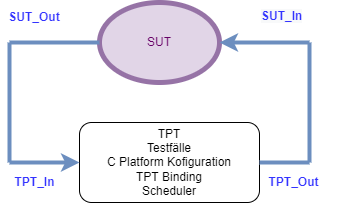
\includegraphics[scale=.6,]{Bilder/Quicktest/SUT_TPT.drawio.png}
\newpage
\section*{\textit{Platform Configuration} und \textit{Platform Execution}}
%zuerst Platform Configuration und Platform Execution und danach C Platform Konfiguration als Überschriften
%Was macht man in der Platform Configuration? Frage beantworten
% Man wählt eine Plattform aus der Plattformkonfiguration aus und 
% In der Plattformkonfiguration 
% Es gibt verschiedene Plattformen, in denen 
Die Plattformkonfigurationen in TPT dienen dazu, das zu testende System in TPT für die Analyse zu konfigurieren.
Eine Plattform ist die C-Platfform, die in dieser Arbeit ausschließlich behandelt wird.
% Es gibt in TPT Plattformen, in denen
% In der Plattformkonfiguration werden 
%Die beiden sind streng getrennt und unabhängig voneinander. Neben der C-Platform Konfiguration gibt es auch noch andere Platformen,
%die aber für diese Arbeit nicht weiter wichtig sind. 
%Es gibt verschiedene Platformkonfigurationen wie beispielsweise die C Platform Konfiguration. 
In der Plattform \textit{Execution} wird festgelegt, welche Tests durchgeführt werden sollen.
Die Plattform Konfiguration und die Plattform \textit{Execution} sind streng getrennt und unabhängig voneinander.
Der große Vorteil dieser Trennung ist, dass die Plattformkonfiguration ausgetauscht werden kann und die Testfälle nicht neu geschrieben
werden müssen. Alle Einstellungen der Plattformkonfiguration sind unabhängig von der Testfallerstellung\cite[vgl.][S. 120]{tpt}. 

\section*{C-Plattform Konfiguration}
%es gibt verschiedene voreingestellte Platformen, die man benutzen kann.
Es gibt folgende Konfigurationsmöglichkeiten \cite[vgl.][S. 862 ff.]{userguide}:
\begin{description}
\item[Compiler auswählen] Pfad zu einem installierten Compiler
\item[Sourcen auswählen] Diese werden später gelinkt und kompiliert, zu analysierende Sourcen müssen auf analysieren gestellt werden
% dabei werden die ausgewählten Sourcen kompiliert und diejenigen, die auf zu analysieren gestellt sind, werden analysiert
% für GSIL: alle \_Task.c auf set analyze setzen
\item[Scheduler] Ein (Prozess-)Scheduler berechnet und entscheidet, wann und wie lange ein Prozess die CPU Zeit bekommt \cite[vgl.][S. 44]{scheduler}.
Hier ist ein Prozess eine Funktion, die ausgeführt wird, sobald sie die CPU Zeit bekommt. %Wenn diese Funktion die CPU Zeit, wird diese ausgeführt. Im 
Im TPT Scheduler werden vom Benutzer Funktionen ausgewählt, die während der Testdurchführung ausgeführt werden sollen.
Es können die ausgewählten Funktionen auf \textit{Startup, Initial} und \textit{Periodic} gestellt werden.
Mit \textit{Startup} wird die Funktion nur einmal am Anfang der Testdurchführung ausgeführt. Mit \textit{Initial} wird die Funktion
einmal am Anfang eines Zyklus ausgeführt und mit \textit{Periodic} wird die Funktion einmal pro definierter Abtastrate ausgeführt.
% Dabei gibt es Startup, wobei die 
% Funktionen, die aufgerufen werden sollen. Hier ist ein Scheduler erklärt \cite{scheduler}.
\item[Step size] die Abtastrate. Gibt beispielsweise die Zeiteinheit der periodischen Scheduler Funktionen an.
\end{description}
%Test execution und test assessment Oberpunkt weiter nach unten
\section*{\textit{Test Execution} und \textit{Test Assessment}}
Die \textit{Test Execution} und das \textit{Test Assessment} sind zwei getrennte Prozesse.  
Die \textit{Test Execution} ist dafür zuständig die Testfälle auszuführen und dabei Daten zu sammeln. % \cite[S. 1212 ff.]{userguide}.
Diese gesammelten Daten werden beim \textit{Test Assessment} ausgewertet. 
Daten sind beispielsweise die Werte der Signale, wobei wichtig sein kann, wann und wie lange ein  bestimmter Wert des Signals überschritten wurde \cite[vgl.][S. 1212 ff.]{userguide}.
Ein Assessment ist beispielsweise die Auswertung eines Compare Steps.
%, es gibt noch folgende weitere Assessments:
Es gibt auch ein Assessment für Äquivalenzklassen. Dabei kann festgelegt werden, welche Äquivalenzklassen erreicht oder auch nicht erreicht werden sollen \cite[vgl.][S. 41 ff.]{tpttutorial}.
%Ein weiteres Assessment ist der Min/Max Vergleich, wobei einzelne Signale detailiert beobachtet werden und festgestellt wird, ob und wie lange ein Signal
%in einem definierten Bereich ist.
% \textit{Test Execution} und \textit{Test Assessment} sind streng getrennt und unabhängig voneinander.
%\cite[S.41 ff.]{tpttutorial}%Quelle ist nur über Compare Step und Assessment, nicht über Min Max
%Während der \textit{Test Execution} werden Daten aufgesammelt. 
%Daten sind beispielsweise die Werte der Signale im Laufe der Zeit des Tests.
%könnten sein, welche Werte Signale zu welcher Zeit angenommen haben oder welcher Systemzustand gerade aktiv ist.
%Diese Daten werden danach im Assessment ausgewertet. 
% In TPT sind diese beiden streng getrennt. 
% Bei Execution:
% Die Testfälle werden durchgeführt. Die Testfälle sind durch automatons, step lists, Variants definiert.
% Bei der Testdurchführung werden Daten gesammelt.
% Beim Assessment:
% Die gesammelten Daten werden hier ausgewertet. ZB Step list wird ausgewertet.
 % Äquivalenzklasse wird ausgewertet. Die "Check Rules" für die Auswertung werden in 
 % den Assesslets festgelegt.
% In TPT werden Execution und Assessment getrennt und sind unabhängig voneinander

\section*{Analysieren der Dateien}
Durch das Analysieren werden Signale sowie Funktionen der Dateien TPT bekannt gegeben. Es wird auch TPT Binding genannt \cite[vgl.][S. 870 ff.]{userguide}.
Das Analysieren erfolgt mit einem Parser. 
Die Aufgabe eines Parsers ist es, Daten auf Korrektheit in Bezug auf einer \glqq Grammatik\grqq{} zu untersuchen und in einer definierten
Struktur intern weiterzuverarbeiten \cite[vgl.][S. 1 ff.]{parser}.
%In einem sogenannten TPT Binding werden die Funktionen vom Scheduler sowie die Signale, in TPT Channels genannt, zusammengestellt.
% Channels können auch in TPT importiert werden
% Hier werden Funktionen mit TPT verbunden. Insbesondere können die Channels, die TPT findet,
% übernommen werden oder man importiert die Declarations im Declaration Editor. 

\section*{Generieren und Kompilieren}
Ein Testrahmen wird generiert und inklusive der analysierten Dateien kompiliert.
Neben dem TPT Binding sind auch Scheduling Informationen im Testrahmen zu finden \cite[vgl.][S. 868 ff.]{userguide}.
%Mit dem TPT Binding wird ein Testrahmen erstellt und schließlich kompiliert.
% Es wird ein sogenannter Testrahmen erstellt, in dem alle Informationen über das TPT Binding(Channels und Informationen) 
% beinhaltet sind. Schließlich wird es kompiliert.

\section*{Testfallerstellung}
es gibt folgende Steps in der Step Liste \cite[vgl.][S. 437 ff.]{userguide}:
\begin{description}
\item[Channel Step] Wertzuweisung auf ein Signal
\item[Compare Step] Ein Signal wird durch das Assessment überprüft, ob es eine definierte Bedingung erfüllt
%\item Channel Step
\item[if, while Step] wie in Programmiersprachen (Java, C++)
\item[wait] Damit läuft die Zeit weiter und Signale können überschrieben werden. Mit @ wird die Zeiteinheit auf die Abtastrate gestellt (siehe C-Plattform Konfiguration Step size).
%läuft die Zeit weiter und eine weitere Sequenz startet, mit @ wird die Wartezeit auf die eingestellte Abtastrate gestellt
% wait Befehl ist nötig, sodass die Zeit weiterlaufen kann und ein weitere Sequenz starten kann.
% Damit wird abgewandt, dass ein Channel einen Kurzschluss hat, indem beispielsweise zwei Werte zur gleichen Zeit
% auf den Channel geschrieben werden.
% wait wie lange?
% am besten mit @
% @ ist eine Referenz auf die eingestellte step size.
\end{description}
Neben der Step Liste gibt es auch noch eine Partition Liste. Diese ermöglicht graphisches Erstellen von Testfallen mithilfe von sogenannten Automatons \cite[vgl.][S. 437 ff.]{userguide}.
\section*{\ac{sut}}
In \autoref{fig:SUT_TPT} ist zu sehen, wie das zu testende System mit \ac{tpt} interagiert.
TPT erzeugt im Sinne des Testfalls ein Signal, sendet dieses an das \ac{sut} und
es wird eine Antwort zurück an \ac{tpt} geschickt.
Die Antwort des \ac{sut} wird in \ac{tpt} verarbeitet und gegebenenfalls ein neues Signal an das \ac{sut} geschickt,
wodurch der Zyklus von Neuem beginnt. Es entsteht ein geschlossener Kreis zwischen \ac{sut} und \ac{tpt}.
Dieser Vorgang wird so oft wiederholt, wie es Testfälle gibt \cite[vgl.][]{tptsut}.% wodurch ein geschlossener Kreis entsteht.
\begin{figure}[h]
\centering
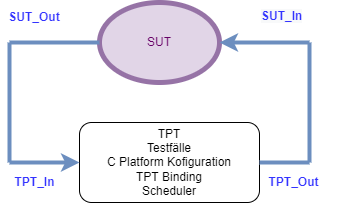
\includegraphics[scale=0.9,]{Bilder/Quicktest/SUT_TPT.drawio.png}
\caption{Zusammenhang zwischen SUT und TPT \cite{tptsut}}\label{fig:SUT_TPT}
\end{figure}

\section*{TPTAPI}
Mithilfe der TPTAPI kann man das komplette Programm steuern. Die \ac{api} ist in Java geschrieben.
In TPT ist Jython installiert, womit man die Java Module in Python verwenden und TPT steuern kann.
Im Listing C.1 im Anhang sind nützliche Funktionen der TPTAPI aufgezählt \cite[vgl.][S. 64 f.]{userguide}.
%Hier werden ein paar nützliche Funktionen vorgestellt:
% \section*{Test Execution und Test Assessment}
% In TPT sind diese beiden streng getrennt. 
% Bei Execution:
% Die Testfälle werden durchgeführt. Die Testfälle sind durch automatons, step lists, Variants definiert.
% Bei der Testdurchführung werden Daten gesammelt.
% Beim Assessment:
% Die gesammelten Daten werden hier ausgewertet. ZB Step list wird ausgewertet.
 % Äquivalenzklasse wird ausgewertet. Die "Check Rules" für die Auswertung werden in 
 % den Assesslets festgelegt.
% In TPT werden Execution und Assessment getrennt und sind unabhängig voneinander

\section*{Äquivalenzklassen}
	% \begin{figure}[h]
% \centering
% 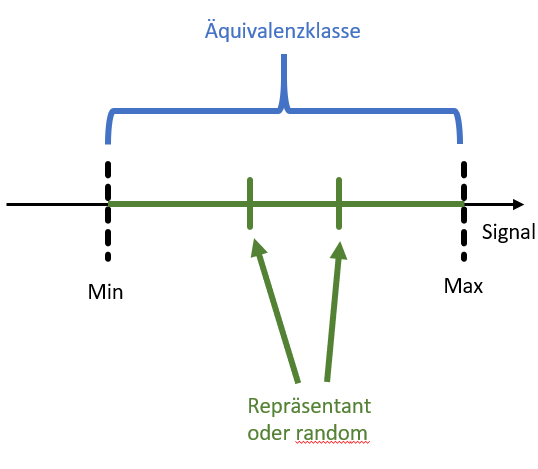
\includegraphics[scale=1.5,]{Bilder/EquiZeitstrahl/ZeitstrahlEineKlasse.png}
% \caption{Äquivalenzklasse in TPT}
% \end{figure}
%\textbf{Darstellung für random, Repräsentanten, Min und Max von Äquivalenzklassen in TPT}
Im \textit{Equivalence Class Set Editor} unter \textit{View} können Äquivalenzklassen definiert werden, um sie 
mehreren Signalen beziehungsweise einem einzigen Signal im Declaration Editor zuzuordnen.
%Die definierten Äquivalenzklassen können im zweiten Schritt Signalen zugeordnet werden.
Sie können als Assesslet \textit{Equivalence Classes} in der Auswertung der Testfälle eingesetzt werden.
%, um zu überprüfen, ob oder ob nicht bestimmte Klassen erreicht werden.
Sie können gleichermaßen in der Step Liste eingesetzt werden, um
Signale auf bestimmte Äquivalenzklassen zu setzen \cite[vgl.][S. 370 ff.]{userguide}.\\
\begin{description}
\item[Assessment]%Ein bild zum Assessment
Mit dem \textit{Equivalence Class Coverage table} können
ausgewählte Testfälle überprüft werden, ob Channels Werte ihrer Äquivalenzklassen
annehmen. In der Report Übersicht wird für jede Äquivalenzklasse der 
gewählten Channels angezeigt, ob und wie oft sie in den gewählten Testfällen vorkommen.
Eine weitere Möglichkeit im Assessment ist, dass 
man forbidden, also verbotene sowie mandatory, verpflichtende
Äquivalenzklassen festlegen kann. Eine Verbotene
besteht den Test, wenn sie nicht eintritt.
Eine Verpflichtende besteht den Test, wenn sie ein
oder mehrere Male eintritt \cite[vgl.][S. 1282 ff.]{userguide}.\\
% Eine verpflichtende Äquivalenzklasse
% kann für ausgewählte 
% Testfälle Channels gesetzt werden. Diese Channels, die Äquivalenzklassen besitzen,
% werden darauf überprüft, ob sie  
% Es wird ein Signal ausgewählt, man kann zwischen mandatory, forbidden und .. auswählen.
% Oben sind 4 Haken zu setzen, diese hier erklären.
\item[Step Liste]%\%ein Bild zur Step Liste
Es gibt vier Schlüsselwörter, um eine Äquivalenzklasse eines Channels
in der Step Liste zu benutzen: \textit{Random, representative, min} und \textit{max}.
Mit \textit{min} und \textit{max} sind jeweils die Grenzen des definierten Wertebereichs gemeint. Mit \textit{random} wird ein zufälliger Wert gewählt, mit \textit{representative} ein Repräsentant.
Wenn kein Schlüsselwort angegeben wird, so wird der Repräsentant gewählt.
Falls kein Repräsentant definiert ist, so wird ein zufälliger Wert innerhalb des Wertebereichs
gewählt \cite[vgl.][S. 379 f.]{userguide}.\\
\item[Äquivalenzklassen von TPT generieren lassen]
Dies kann man mit \textit{Generate Test Cases -> from Equivalence Classes} erreichen.
Man kann auswählen ob sie in einer Step Liste nacheinander
geschrieben werden oder jede in einer 
eigenen Step Liste. Weitere Einstellungsmöglichkeiten sind eine paarweise Kombination und Grenzwerte (siehe Abschnitt 2.2) \cite[vgl.][S. 668 ff.]{userguide}. 
\end{description}
% Generate Test Cases -> from Equivalence Classes 
% Optionen: Auswählen ob Äquivalenzklassen in einzelnen Testfällen, oder alles in einen Testfall als Sequence geschrieben werden

% % Wie erstellt man Äquivalenzklassen in TPT?
% % View -> Equivalence Class Set Editor, Signal in Wertebereich einteilen
% % View -> Declaration Editor Channel(Signal) auf definierte Äquivalenzklasse setzen
% % Assessment -> Equivalence Class auswählen
% % Signale auswählen, mandatory und forbidden equi classes eingeben

% % fertig, jetzt Testdurchführung

% % Äquivalenzklassen von TPT generieren lassen:
% % Generate Test Cases -> from Equivalence Classes 
% % Optionen: Auswählen ob Äquivalenzklassen in einzelnen Testfällen, oder alles in einen Testfall als Sequence geschrieben werden

% % Möglichkeiten der Test Case Erstellung mit Äquivalenzklassen
% % mit Signal.ec->high etc., Repräsentanten und andere Funktionen

% % Dieses Kapitel zu TPT Analyse
		%\newpage
		\chapter{Grundlagen}
			In diesem Kapitel werden die Grundlagen erarbeitet, worauf die Umsetzung basieren wird.
Es wird auf Schnittstellen eingegangen und wie diese gestestet werden können. Ein weiterer Punkt sind
die Äquivalenzklassen. Dabei werden die Äquivalenzklassen mathematisch beschrieben und erklärt, wie sie in 
der Informatik angewandt werden.
 % Zuerst werden diese mathematisch beschrieben und danach wie sie in der Informatik
% eingesetzt werden. 
% Für den Schnittstellentest ein Punkt, für die Äquivalenzklassen.
Die Umsetzung erfolgt in \ac{tpt}, weshalb im Abschnitt 2.3 erklärt wird, welche Funktionalitäten \ac{tpt} hat und wie es 
konfiguriert wird.
			\section{Schnittstellen}
				Ein Teil des Integrationstests ist der Schnittstellentest. Schnittstellen sorgen dafür, dass
Softwareteile, insbesondere Softwarekomponenten miteinander verbunden sind und Daten austauschen können.
Es werden verschiedene Arten von Schnittstellendefinitionen vorgestellt und es wird gezeigt, wie eine 
Schnittstelle getestet werden kann.
In Abbildung 2.1 ist zu sehen, wie zwei Komponenten durch eine Schnittstellendefinition verbunden sind.\par
\begin{figure}[!h]
\centering
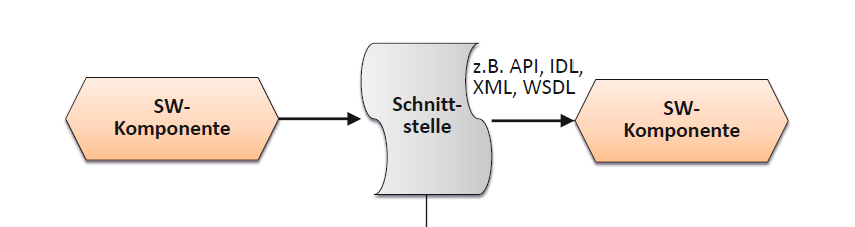
\includegraphics[scale=.9,]{Bilder/Quicktest/Schnittstelle.png}
\caption{Schnittstellen \cite[S.218]{integration}}\label{fig:schnitt}
\end{figure}
Es gibt verschiedene Arten, wie man eine Schnittstelle definieren kann \cite[vgl.][S. 218 ff.]{integration}:
\begin{description}
\item[unstrukturierte Datenübergabe] Es gibt keine feste Schnittstellendefinition. 
Der Empfänger muss die Daten selbst interpretieren. %Automatisierte Analysen sind kaum möglich.
\item[Gemeinsame globale Datenbereiche] Komponenten können darauf zugreifen, Werte ablegen und entnehmen.
Wenn beide Komponenten jedoch eine eigene Definition des Datentyps haben, wird die Wartbarkeit bei Änderungen
schwierig. Abhilfe kann hier eine Header Datei sein, in der die Datenstruktur definiert ist. Eine Header Datei
dient als Schnittstelle zwischen Dateien. Damit können Daten für mehrere Dateien sichtbar gemacht werden.
\item[\ac{api}] Daten werden über eine \ac{api} übertragen. Dabei werden die Daten 
in einen Stapel gespeichert und an die Zielkomponente übergeben, welche die Daten vom Stapel entpackt. Es kann
ein Rückgabewert (Return) an die Senderkomponente zurückgesendet werden.
%Dateien später bei xml, sql bla bla
\item[Datenbanken] Der Datenaustausch ist über eine gemeinsame Datenbank definiert. Die erste Komponente legt
Daten ab, die zweite Komponente holt die Daten. Datenbanken
werden oft in IT-Systemen eingesetzt.
Der Test einer Datenbank kann erfolgen, indem Dateninhalte überprüft werden. Es bietet sich auch an, die Datenbank
zu manipulieren, indem einzelne Zeilen oder Spalten verändert werden, um die Auswirkungen zu überprüfen.
\item[Schnittstellendefinitionssprachen] Sie haben die Aufgabe eine sichere Datenübertragung
zu ermöglichen, indem die Struktur der zu sendenden Daten klar definiert wird.
Eine Schnittstellendefinitionssprache ist \ac{xml}. In einem Schema wird die 
Struktur und der Inhalt der Schnittstelle festgelegt. Anhand dieses Schemas wird überprüft, ob die Daten richtig sind.
Ein Vorteil von \ac{xml} ist, dass es einfach erweiterbar ist. Es ist auch sehr flexibel, sodass eine Schema nach
den eigenen Bedingungen erstellt werden kann. Es ist sinnvoll, strenge Regeln aufzustellen, damit eine Überprüfung besser
möglich ist.
\end{description}


\section*{Schnittstellentest}
Für den Schnittstellentest benötigt es zwei Schritte, wie in Abbildung 2.2 zu sehen ist.
Ein Schritt ist, dass getestet wird, ob das Format der Schnittstellendefinition eingehalten wird.
Ein Entwickler schreibt die Schnittstelle und die Überprüfung erfolgt von einer zweiten Person. Der Überprüfer hat einen
anderen Blickwinkel und kann Denkfehler besser erkennen und sofort lösen \cite[vgl.][S. 226]{integration}.
Als Beispiel einer Schnittstelle wird im Folgenden \ac{xml} genommen.
Es gibt automatisierte Tests wie einen XML-Analysator. Dieser überprüft XML-Daten gegen die Struktur im vorgegebenen
Schema \cite[vgl.][S. 237]{integration}.

Damit werden nur die XML-Daten an sich überprüft. Ein zweiter wichtiger Punkt ist die Überprüfung des Zugriffs auf die Daten, die in einer XML hinterlegt sind.
Dafür muss der Code geprüft werden, in der die Schnittstelle verwendet wird.
Die Schnittstelle wird auf Empfänger- und Senderseite überprüft. Dabei können Parameter wie der Typ, die Reihenfolge oder die Nutzungsart eine Rolle spielen \cite[vgl.][S. 228]{integration}.\par
\begin{figure}[!h]
\centering
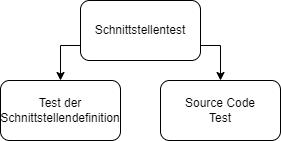
\includegraphics[scale=.9,]{Bilder/Quicktest/Schnittstellen.drawio.png}
\caption{Schnittstellentest \cite[vgl.][S. 226]{integration}}
\end{figure}














% Die Schnittstelle wird auf den Typ, die Reihenfolge, die Nutzungsart
% % die Parameter der Schnittstellendefinition, den Typ, die Reihenfolge, die Nutzungsart
% mit den Ein-/Ausgabe-Operationen geprüft.

 % Die Schnittstelle soll gelesen und geprüft werden.
% Es kann ein sogenanntes Review machen. Einer  
% Dies kann mit einem XML-Analysator überprüft werden. 
% Ein zweiter Schritt ist, dass der Source Code getestet wird, ob diese Schnittstelle richtig angewandt wird.\par


% die Schnittstellendefinition überprüft werden.
% Zum Anderen muss der Source Code überprüft werden, ob diese Schnittstelle richtig gemacht wird.
% Bild: Test Schnittstellen 
% Überprüfung Schnittstellendefinition, zweiter Punkt Abgleich (Baustein A, Baustein B) Seite 226

% Beim Abgleich:
% Informationen aus xml.
% Code wird überprüft, ob Informationen aus xml im Code richtig geschrieben wurden.
% "wird der Source Code der Schnittstelle gelesen und geprüft, ob die Parameter der Schnittstellen-
% definition in der Anzahl, im Typ, in der Reihenfolge und in der Nutzungsart mit den
% Ein/Ausgabe Operationen der Sender und Empfänger der Schnittstelle übereinstimmen"(dh ob die Daten, die in der
% xml über die Schnittstelle definiert wurden, im Code richtig eingesetzt wurden.)

% Bei ZF ist es so:
% Schnittstellen inklusive Signale in xml.
% Code in C geschrieben: Verbindung von zwei Signalen in C Code geschrieben, durch Einsetzen der Makros
% Makros, Header Dateien aus xml generiert.

% Quicktest bei ZF:(das ist genau dieser Abgleich)
% Überprüfen, ob der per Hand geschriebene C Code die Schnittstelle, so wie sie in xml definiert ist,
% richtig abbildet.

% dann zu beiden Punkten noch was schreiben





% 12.1.x aufzählen
% Schnittstellen Review

% Bild auf Seite 231 ist auch gut.
% 12.2 Ansätze für Tests ab Seite 225

% eine Lösung ist statische Schnittstellenanalyse
			\section{Äquivalenzklassentest}%mathematische Grundlagen Äquivalenzklassentest
				%Äquivalenzklassen gibt es schon seit bla bla. Äquivalenzklassen finden jetzt auch in der Informatik Anwendung. bla bla
In diesem Punkt geht es um die Äquivalenzklassen. Sie werden mathematisch beschrieben und danach wird gezeigt, wie sie
in der Informatik Anwendung finden.
\section*{Mathematische Beschreibung der Äquivalenzklassen}
Seien zwei Elemente zu einer Teilmenge R zugeordnet, so spricht man von einer Relation der beiden Elemente und schreibt $\sim$. 
Eine Äquivalenzrelation liegt vor, wenn eine Relation reflexiv, symmetrisch und 
transitiv ist, wie in Abbildung 2.3 dargestellt.
Eine reflexive Relation ist gegeben, wenn jedes Element einer Menge in Relation zu sich selbst steht. %(https://de.wikipedia.org/wiki/Reflexive_Relation, Abruf 14.04.22 14:%$ uhr)
Eine symmetrische Relation ist gegeben, wenn zwei Elemente einer Menge gegeneinander austauschbar sind, wobei die Relation zueinander gegeben bleibt.
%Transitive Relation bedeutet, dass die Relation zweier Elemente auf ein drittes Element übertragbar ist, sofern
Eine transitive Relation ist gegeben, wenn ein Element in Relation zu zwei anderen Elementen steht, so stehen jene beide Elemente auch in Relation zueinander \parencite[S. 66]{equimaths}.
\begin{figure}[!h]
\centering
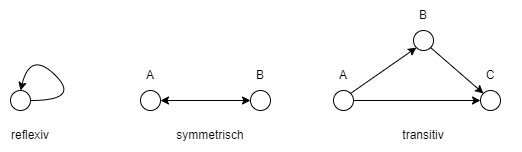
\includegraphics[scale=.9,]{Bilder/EquiDrawio/EigenschaftenEqui.drawio.png}
\caption{Eigenschaften einer Äquivalenzklasse \parencite{eigequi1}\parencite{eigequi2}}
\end{figure}
\newpage
\paragraph{Definition der Äquivalenzklasse}
$$[a] = \{b \in M ; b \sim a\}$$
\begin{center}
bezeichnet man als Äquivalenzklasse des Elements $a$ in $M$,\\
wobei $\sim$ eine Äquivalenzrelation auf einer Menge $M$ ist und\\
\end{center}
$$a,b \in M.$$
Alle Elemente einer Äquivalenzrelation in der Gesamtheit bezeichnet man als Äquivalenzklasse.
Jedes einzelne Element davon bezeichnet man als Repräsentanten der Äquivalenzklasse \parencite[S. 66]{equimaths}.

\section*{Äquivalenzklassen in der Informatik}
Um den Bezug zur Informatik herzustellen, wird als Menge der Wertebereich eines Parameters bezeichnet.
Das Prinzip der Äquivalenzklassen kann so auf Parameter angewendet werden, indem ein Parameter in Wertebereiche eingeteilt wird, wie es in Abbildung 2.4 zu sehen ist.
Ein Repräsentant einer Äquivalenzklasse ist ein beliebiger Wert innerhalb des Wertebereichs. 
Es ist gewollt, dass auch Äquivalenzklassen definiert werden, die ein kritisches oder fehlerhaftes Verhalten des Systems erzeugen können.
Wie sie im Detail definiert werden, soll aus dem Requirement hervorgehen.
Sie werden so gewählt, dass sich das System für alle Werte innerhalb der Äquivalenzklasse gleich/ähnlich verhält. Somit reicht es aus, nur 
einen Repräsentanten zu testen. 
Der Sinn der Äquivalenzklassen ist es, dass redundante Testfälle vermieden werden, indem jeweils nur Repräsentanten getestet werden.
Die Anzahl der Testfälle entsteht durch das Produkt aller Äquivalenzklassen pro Parameter. Bei mehreren Parametern sowie der dazugehörigen definierten Wertebereiche
können schnell viele Testfälle entstehen \parencite[S. 114 ff.]{equiinformatic}.\par
\begin{figure}[h]
\centering
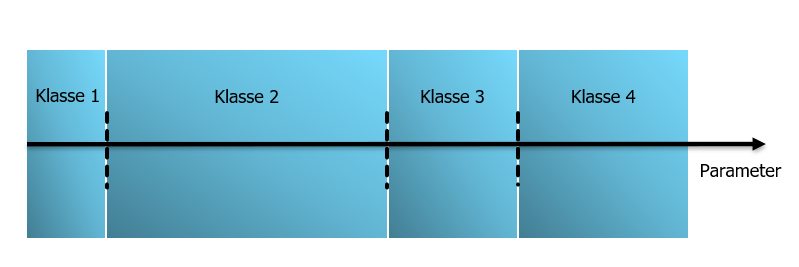
\includegraphics[scale=1.2,]{Bilder/EquiZeitstrahl/ZeitstrahlVerschiedeneKlassenParameter.png} %,6 für VerschieneKlassen
\caption{Einteilung eines Parameters in Äquivalenzklassen \parencite[S. 114 ff.]{equiinformatic}}
\end{figure}
Möglichkeiten der Testfalleinschränkung \parencite[S. 120]{equiinformatic}:
\begin{itemize}
\item Testfälle filtern, dass nur oft vorkommende Kombinationen getestet werden
\item Testfälle mit Grenzwerten bevorzugen
\item paarweise Kombination: jeweils zwei Repräsentanten unterschiedler Äquivalenzklassen werden kombiniert
\item Minimalkriterium: jeder Repräsentant ist in mindestens einem Testfall vorhanden
\item Repräsentanten, die ein kritisches/fehlerhaftes Verhalten hervorrufen, werden nicht miteinander kombiniert
\end{itemize}

%Ungültige Äquivalenzklasse bezieht sich darauf, dass es eine Äquivalenzklasse ist, die ein kritisches/fehlerhaftes Verhalten hervorrufen soll.
% (Ausgangskriterium:\\
% ÄK-Überdeckung = ( getestete ÄK / alle ÄK ) x 100\%) \parencite[S.114 ff.]{equiinformatic}







































% (
% "
% Sicherstellen, dass jeder Repräsentant einer Äquivalenzklasse mit
% jedem Repräsentanten der anderen Äquivalenzklassen in einem
% Testfall zur Ausführung kommt (d. h. paarweise Kombination
% statt vollständiger Kombination)."
% Verbesserung:
% "Als Minimalkriterium sicherstellen, dass jeder Repräsentant einer
% Äquivalenzklasse in mindestens einem Testfall vorkommt."

% "Es werden allerdings nur einzelne Ein- oder Ausgabebedingungen
% betrachtet, mögliche Abhängigkeiten oder Wechselwirkungen zwischen
% den Bedingungen werden nicht berücksichtigt bzw. sind sehr
% aufwendig zu berücksichtigen (durch weitere Aufteilung der Äquivalenzklassen
% und entsprechende Kombinationen)."
% )

% reflexiv:\\
% 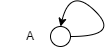
\includegraphics[scale=.9,]{Bilder/EquiDrawio/reflexiv.drawio.png}
% symmetrisch:\\
% 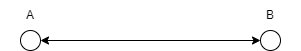
\includegraphics[scale=.9,]{Bilder/EquiDrawio/symmetrisch.drawio.png}
% transitiv:\\
% 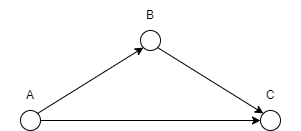
\includegraphics[scale=.9,]{Bilder/EquiDrawio/transitiv.drawio.png}
% \textbf{Bildinfo 3 Bilder reflexiv etc: 3 Eigenschaften von Äquivalenzklassen}

% \begin{figure}[!h]
% \centering
% 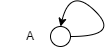
\includegraphics[scale=.9,]{Bilder/EquiDrawio/reflexiv.drawio.png}
% \caption{reflexiv}
% \end{figure}

% \begin{figure}[!h]
% \centering
% 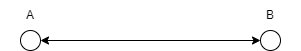
\includegraphics[scale=.9,]{Bilder/EquiDrawio/symmetrisch.drawio.png}
% \caption{symmetrisch}
% \end{figure}

% \begin{figure}[!h]
% \centering
% 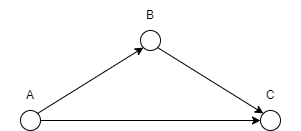
\includegraphics[scale=.9,]{Bilder/EquiDrawio/transitiv.drawio.png}
% \caption{transitiv}
% \end{figure}
			\section{Konfiguration von TPT}
				In Abbildung 2.5 ist ein Überblick zu sehen, welche Schritte nötig sind, um TPT für einen Test einzurichten \cite[vgl.][S. 39]{userguide}. 
%Im Folgenden ist zu sehen, welche Schritte benötigt werden, um TPT für einen Test einzurichten:
\begin{figure}[!h]
    \centering


  \begin{tikzpicture}%[every node/.style={rectangle,draw,text width=14em,align=center}]
    [
      % Stil für Ein- und Ausgabe
      io/.style={trapezium, trapezium left angle=70, trapezium right angle=110, fill=magenta!10, draw=magenta},
      % Stil für Operationen
      op/.style={rectangle, fill=orange!10, draw=orange},
      op4/.style={rectangle, fill=green!20, draw=green},
			op2/.style={rectangle, fill=green!20, draw=green, minimum height=2cm, minimum width=38mm},
			op3/.style={rectangle, fill=orange!10, draw=orange, minimum height=2cm, minimum width=38mm},
      % Stil für Entscheidungen
      cn/.style={diamond, aspect=2, inner sep=1pt, fill=red!10, draw=red, minimum width=20mm, minimum height=14mm},
      cn2/.style={diamond, aspect=2, inner sep=1pt, fill=blue!20, draw=blue, minimum width=20mm, minimum height=14mm},% Distanz zwischen den Knoten
      node distance=4mm]
    % Knoten
    %\node[op4] (class) {GSIL Projekt als Ausgang};
    
    \node[op4] (init) {C-Plattform Konfiguration};
    \node[op4, below=of init] (list) {Analysieren der Dateien};
    %\node[op, below=of list] (firstitem) {select first item in list};
%    \node[cn2, below=of list] (cond1) {};
    \node[op4, below=of list] (compile) {Generieren des TPT Testrahmens und Kompilieren};
    \node[op4, below=of compile] (depnewlist) {Testfallerstellung};
    \node[op4, below=of depnewlist] (execution) {\textit{Execution} Konfiguration};
    \node[op4, below=of execution] (final) {Testdurchführung};
%    \node[cn2, below=of depnewlist] (cond2) {};
    %\node[op, right=of cond2] (wrongdep) {select next item};
    %\node[op, below=of cond2] (makefiles) {search for item in dictionary to get makefiles};
    % \node[op4, below=of cond2] (initdep) {initialize object using item};
    % \node[op4, below=of initdep] (addobject) {add to object list};
    % \node[cn2, below=of addobject] (cond3) {\shortstack{last item from \\ dependency list?}};
    % \node[op4, right=of cond3] (wrongdep) {select next item};
    % \node[op4, below=of cond3] (findsubs) {object.findSubdirectories()};
    % \node[op4, below=of findsubs] (findfiles) {object.findFiles()};
    % \node[cn2, below=of findfiles] (cond4) {\shortstack{last item from\\ object list?}};
    % \node[op4, left=of cond4] (wrongobject) {select next item};
    % \node[op4, below=of cond4] (end) {Ende};
    
    \path[->]
		%(class) edge (init)
		(init) edge (list)
		(list) edge (compile)
		(compile) edge (depnewlist)
		(depnewlist) edge (execution)
		(execution) edge (final);
      % (finddep) edge (depnewlist)
      % (depnewlist) edge (cond2)
      % (cond2) edge (initdep)
      % (initdep) edge (addobject)
      % (addobject) edge (cond3)
      % (cond3) edge node[above=0.2cm] {No}(wrongdep)
      % (cond3) edge node[right=0.2cm] {Yes} (findsubs)
      % (findsubs) edge (findfiles)
			% (findfiles) edge (cond4)
      % (cond4) edge node[above=0.2cm] {No}(wrongobject)
      % (cond4) edge node[left=0.5cm] {Yes} (end);

    % \draw[->] 
      % (wrongdep) --  ++(2,0) |- (cond2)
      % (wrongobject) -- ++(-2,0) |- (cond1);
		% \draw[->] (cond2) -- node[below] {Nein} ++(2.9,0) -- (entscheid);
		% \draw[->] (cond4) -- node[below] {Nein} ++(4.0,0) -| (gescheitert2);
		% \draw[->] (cond3) -- node[below] {Nein} ++(-4.0,0) -| (gescheitert3);
      %(wrongdep) edge (cond1);
			% (cond1) edge node[right] {Ja} (cond2)
			% (cond2) edge node[below] {Ja} (gesetz2);
    
    % \node[cn, align=center, below=of begehren] (cond1) {okay\\Unterschriften?};
		% \node[cn, align=center, below=of cond1] (cond2) {Landtag nimmt\\Gesetzentwurf an?};
		% \node[op3, align=center, right=of cond1] (gescheitert) {Volksbegehren\\gescheitert};
		% \node[op, align=center, right=of cond2] (entscheid) {Volksentscheid};
		% \node[io, below=of entscheid] (abstimmung) {Stimmen Sie ab!};
		% \node[cn, align=center, below=of abstimmung] (cond3) {Mehrheit stimmt\\mit Ja?};
		% \node[cn, align=center, below=of cond3] (cond4) {Mehr als ein Drittel\\aller Stimmberechtigten\\ stimmt mit Ja?};
		% \node[op2, align=center, below=of cond4] (gesetz) {Gesetz};
		% \node[op3, align=center, right=of gesetz] (gescheitert2) {Volksbegehren\\gescheitert};
		% \node[op3, align=center, left=of gesetz] (gescheitert3) {Volksbegehren\\gescheitert};
		% \node[op2, align=center, left=of cond2] (gesetz2) {Gesetz};
    % % Kanten
    % \path[->]
    %   (begehren) edge (cond1)
		% 	(entscheid) edge (abstimmung)
		% 	(abstimmung) edge (cond3)
    %   (cond3) edge node[right] {Ja} (cond4)
		% 	(cond4) edge node[right] {Ja} (gesetz)
		% 	(cond1) edge node[right] {Ja} (cond2)
		% 	(cond2) edge node[below] {Ja} (gesetz2);

    % \draw[->] (cond1) -- node[below] {Nein} ++(2.8,0) -- (gescheitert);
		% \draw[->] (cond2) -- node[below] {Nein} ++(2.9,0) -- (entscheid);
		% \draw[->] (cond4) -- node[below] {Nein} ++(4.0,0) -| (gescheitert2);
		% \draw[->] (cond3) -- node[below] {Nein} ++(-4.0,0) -| (gescheitert3);

  \end{tikzpicture}
  \caption{Flussdiagramm TPT Einrichtung \parencite[S. 39]{userguide}}
  \end{figure}

%\textbf{Bildinfo Implementierung Quicktest: Überblick, was man in TPT alles für den Quicktest einstellen muss}

% \section*{Testfallerstellung}
% \section*{C Platform Konfiguration}
% Scheduler, TPT Binding, Auswahl der Sourcen, import interface?, Compiler

% großes grünes Flussdiagrammweg
%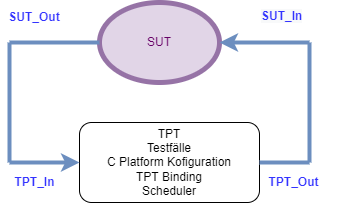
\includegraphics[scale=.6,]{Bilder/Quicktest/SUT_TPT.drawio.png}
\newpage
\section*{\textit{Platform Configuration} und \textit{Platform Execution}}
%zuerst Platform Configuration und Platform Execution und danach C Platform Konfiguration als Überschriften
%Was macht man in der Platform Configuration? Frage beantworten
% Man wählt eine Plattform aus der Plattformkonfiguration aus und 
% In der Plattformkonfiguration 
% Es gibt verschiedene Plattformen, in denen 
Die Plattformkonfigurationen in TPT dienen dazu, das zu testende System in TPT für die Analyse zu konfigurieren.
Eine Plattform ist die C-Platfform, die in dieser Arbeit ausschließlich behandelt wird.
% Es gibt in TPT Plattformen, in denen
% In der Plattformkonfiguration werden 
%Die beiden sind streng getrennt und unabhängig voneinander. Neben der C-Platform Konfiguration gibt es auch noch andere Platformen,
%die aber für diese Arbeit nicht weiter wichtig sind. 
%Es gibt verschiedene Platformkonfigurationen wie beispielsweise die C Platform Konfiguration. 
In der Plattform \textit{Execution} wird festgelegt, welche Tests durchgeführt werden sollen.
Die Plattform Konfiguration und die Plattform \textit{Execution} sind streng getrennt und unabhängig voneinander.
Der große Vorteil dieser Trennung ist, dass die Plattformkonfiguration ausgetauscht werden kann und die Testfälle nicht neu geschrieben
werden müssen. Alle Einstellungen der Plattformkonfiguration sind unabhängig von der Testfallerstellung\cite[vgl.][S. 120]{tpt}. 

\section*{C-Plattform Konfiguration}
%es gibt verschiedene voreingestellte Platformen, die man benutzen kann.
Es gibt folgende Konfigurationsmöglichkeiten \cite[vgl.][S. 862 ff.]{userguide}:
\begin{description}
\item[Compiler auswählen] Pfad zu einem installierten Compiler
\item[Sourcen auswählen] Diese werden später gelinkt und kompiliert, zu analysierende Sourcen müssen auf analysieren gestellt werden
% dabei werden die ausgewählten Sourcen kompiliert und diejenigen, die auf zu analysieren gestellt sind, werden analysiert
% für GSIL: alle \_Task.c auf set analyze setzen
\item[Scheduler] Ein (Prozess-)Scheduler berechnet und entscheidet, wann und wie lange ein Prozess die CPU Zeit bekommt \cite[vgl.][S. 44]{scheduler}.
Hier ist ein Prozess eine Funktion, die ausgeführt wird, sobald sie die CPU Zeit bekommt. %Wenn diese Funktion die CPU Zeit, wird diese ausgeführt. Im 
Im TPT Scheduler werden vom Benutzer Funktionen ausgewählt, die während der Testdurchführung ausgeführt werden sollen.
Es können die ausgewählten Funktionen auf \textit{Startup, Initial} und \textit{Periodic} gestellt werden.
Mit \textit{Startup} wird die Funktion nur einmal am Anfang der Testdurchführung ausgeführt. Mit \textit{Initial} wird die Funktion
einmal am Anfang eines Zyklus ausgeführt und mit \textit{Periodic} wird die Funktion einmal pro definierter Abtastrate ausgeführt.
% Dabei gibt es Startup, wobei die 
% Funktionen, die aufgerufen werden sollen. Hier ist ein Scheduler erklärt \cite{scheduler}.
\item[Step size] die Abtastrate. Gibt beispielsweise die Zeiteinheit der periodischen Scheduler Funktionen an.
\end{description}
%Test execution und test assessment Oberpunkt weiter nach unten
\section*{\textit{Test Execution} und \textit{Test Assessment}}
Die \textit{Test Execution} und das \textit{Test Assessment} sind zwei getrennte Prozesse.  
Die \textit{Test Execution} ist dafür zuständig die Testfälle auszuführen und dabei Daten zu sammeln. % \cite[S. 1212 ff.]{userguide}.
Diese gesammelten Daten werden beim \textit{Test Assessment} ausgewertet. 
Daten sind beispielsweise die Werte der Signale, wobei wichtig sein kann, wann und wie lange ein  bestimmter Wert des Signals überschritten wurde \cite[vgl.][S. 1212 ff.]{userguide}.
Ein Assessment ist beispielsweise die Auswertung eines Compare Steps.
%, es gibt noch folgende weitere Assessments:
Es gibt auch ein Assessment für Äquivalenzklassen. Dabei kann festgelegt werden, welche Äquivalenzklassen erreicht oder auch nicht erreicht werden sollen \cite[vgl.][S. 41 ff.]{tpttutorial}.
%Ein weiteres Assessment ist der Min/Max Vergleich, wobei einzelne Signale detailiert beobachtet werden und festgestellt wird, ob und wie lange ein Signal
%in einem definierten Bereich ist.
% \textit{Test Execution} und \textit{Test Assessment} sind streng getrennt und unabhängig voneinander.
%\cite[S.41 ff.]{tpttutorial}%Quelle ist nur über Compare Step und Assessment, nicht über Min Max
%Während der \textit{Test Execution} werden Daten aufgesammelt. 
%Daten sind beispielsweise die Werte der Signale im Laufe der Zeit des Tests.
%könnten sein, welche Werte Signale zu welcher Zeit angenommen haben oder welcher Systemzustand gerade aktiv ist.
%Diese Daten werden danach im Assessment ausgewertet. 
% In TPT sind diese beiden streng getrennt. 
% Bei Execution:
% Die Testfälle werden durchgeführt. Die Testfälle sind durch automatons, step lists, Variants definiert.
% Bei der Testdurchführung werden Daten gesammelt.
% Beim Assessment:
% Die gesammelten Daten werden hier ausgewertet. ZB Step list wird ausgewertet.
 % Äquivalenzklasse wird ausgewertet. Die "Check Rules" für die Auswertung werden in 
 % den Assesslets festgelegt.
% In TPT werden Execution und Assessment getrennt und sind unabhängig voneinander

\section*{Analysieren der Dateien}
Durch das Analysieren werden Signale sowie Funktionen der Dateien TPT bekannt gegeben. Es wird auch TPT Binding genannt \cite[vgl.][S. 870 ff.]{userguide}.
Das Analysieren erfolgt mit einem Parser. 
Die Aufgabe eines Parsers ist es, Daten auf Korrektheit in Bezug auf einer \glqq Grammatik\grqq{} zu untersuchen und in einer definierten
Struktur intern weiterzuverarbeiten \cite[vgl.][S. 1 ff.]{parser}.
%In einem sogenannten TPT Binding werden die Funktionen vom Scheduler sowie die Signale, in TPT Channels genannt, zusammengestellt.
% Channels können auch in TPT importiert werden
% Hier werden Funktionen mit TPT verbunden. Insbesondere können die Channels, die TPT findet,
% übernommen werden oder man importiert die Declarations im Declaration Editor. 

\section*{Generieren und Kompilieren}
Ein Testrahmen wird generiert und inklusive der analysierten Dateien kompiliert.
Neben dem TPT Binding sind auch Scheduling Informationen im Testrahmen zu finden \cite[vgl.][S. 868 ff.]{userguide}.
%Mit dem TPT Binding wird ein Testrahmen erstellt und schließlich kompiliert.
% Es wird ein sogenannter Testrahmen erstellt, in dem alle Informationen über das TPT Binding(Channels und Informationen) 
% beinhaltet sind. Schließlich wird es kompiliert.

\section*{Testfallerstellung}
es gibt folgende Steps in der Step Liste \cite[vgl.][S. 437 ff.]{userguide}:
\begin{description}
\item[Channel Step] Wertzuweisung auf ein Signal
\item[Compare Step] Ein Signal wird durch das Assessment überprüft, ob es eine definierte Bedingung erfüllt
%\item Channel Step
\item[if, while Step] wie in Programmiersprachen (Java, C++)
\item[wait] Damit läuft die Zeit weiter und Signale können überschrieben werden. Mit @ wird die Zeiteinheit auf die Abtastrate gestellt (siehe C-Plattform Konfiguration Step size).
%läuft die Zeit weiter und eine weitere Sequenz startet, mit @ wird die Wartezeit auf die eingestellte Abtastrate gestellt
% wait Befehl ist nötig, sodass die Zeit weiterlaufen kann und ein weitere Sequenz starten kann.
% Damit wird abgewandt, dass ein Channel einen Kurzschluss hat, indem beispielsweise zwei Werte zur gleichen Zeit
% auf den Channel geschrieben werden.
% wait wie lange?
% am besten mit @
% @ ist eine Referenz auf die eingestellte step size.
\end{description}
Neben der Step Liste gibt es auch noch eine Partition Liste. Diese ermöglicht graphisches Erstellen von Testfallen mithilfe von sogenannten Automatons \cite[vgl.][S. 437 ff.]{userguide}.
\section*{\ac{sut}}
In \autoref{fig:SUT_TPT} ist zu sehen, wie das zu testende System mit \ac{tpt} interagiert.
TPT erzeugt im Sinne des Testfalls ein Signal, sendet dieses an das \ac{sut} und
es wird eine Antwort zurück an \ac{tpt} geschickt.
Die Antwort des \ac{sut} wird in \ac{tpt} verarbeitet und gegebenenfalls ein neues Signal an das \ac{sut} geschickt,
wodurch der Zyklus von Neuem beginnt. Es entsteht ein geschlossener Kreis zwischen \ac{sut} und \ac{tpt}.
Dieser Vorgang wird so oft wiederholt, wie es Testfälle gibt \cite[vgl.][]{tptsut}.% wodurch ein geschlossener Kreis entsteht.
\begin{figure}[h]
\centering
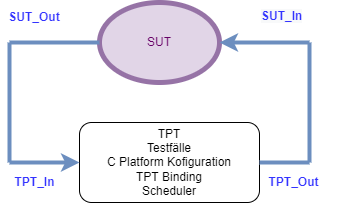
\includegraphics[scale=0.9,]{Bilder/Quicktest/SUT_TPT.drawio.png}
\caption{Zusammenhang zwischen SUT und TPT \cite{tptsut}}\label{fig:SUT_TPT}
\end{figure}

\section*{TPTAPI}
Mithilfe der TPTAPI kann man das komplette Programm steuern. Die \ac{api} ist in Java geschrieben.
In TPT ist Jython installiert, womit man die Java Module in Python verwenden und TPT steuern kann.
Im Listing C.1 im Anhang sind nützliche Funktionen der TPTAPI aufgezählt \cite[vgl.][S. 64 f.]{userguide}.
%Hier werden ein paar nützliche Funktionen vorgestellt:
% \section*{Test Execution und Test Assessment}
% In TPT sind diese beiden streng getrennt. 
% Bei Execution:
% Die Testfälle werden durchgeführt. Die Testfälle sind durch automatons, step lists, Variants definiert.
% Bei der Testdurchführung werden Daten gesammelt.
% Beim Assessment:
% Die gesammelten Daten werden hier ausgewertet. ZB Step list wird ausgewertet.
 % Äquivalenzklasse wird ausgewertet. Die "Check Rules" für die Auswertung werden in 
 % den Assesslets festgelegt.
% In TPT werden Execution und Assessment getrennt und sind unabhängig voneinander

\section*{Äquivalenzklassen}
	% \begin{figure}[h]
% \centering
% 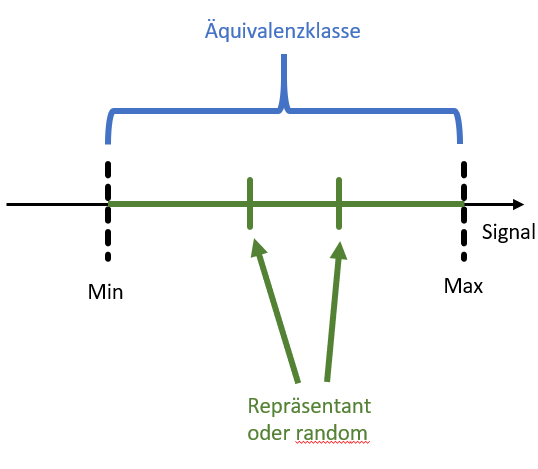
\includegraphics[scale=1.5,]{Bilder/EquiZeitstrahl/ZeitstrahlEineKlasse.png}
% \caption{Äquivalenzklasse in TPT}
% \end{figure}
%\textbf{Darstellung für random, Repräsentanten, Min und Max von Äquivalenzklassen in TPT}
Im \textit{Equivalence Class Set Editor} unter \textit{View} können Äquivalenzklassen definiert werden, um sie 
mehreren Signalen beziehungsweise einem einzigen Signal im Declaration Editor zuzuordnen.
%Die definierten Äquivalenzklassen können im zweiten Schritt Signalen zugeordnet werden.
Sie können als Assesslet \textit{Equivalence Classes} in der Auswertung der Testfälle eingesetzt werden.
%, um zu überprüfen, ob oder ob nicht bestimmte Klassen erreicht werden.
Sie können gleichermaßen in der Step Liste eingesetzt werden, um
Signale auf bestimmte Äquivalenzklassen zu setzen \cite[vgl.][S. 370 ff.]{userguide}.\\
\begin{description}
\item[Assessment]%Ein bild zum Assessment
Mit dem \textit{Equivalence Class Coverage table} können
ausgewählte Testfälle überprüft werden, ob Channels Werte ihrer Äquivalenzklassen
annehmen. In der Report Übersicht wird für jede Äquivalenzklasse der 
gewählten Channels angezeigt, ob und wie oft sie in den gewählten Testfällen vorkommen.
Eine weitere Möglichkeit im Assessment ist, dass 
man forbidden, also verbotene sowie mandatory, verpflichtende
Äquivalenzklassen festlegen kann. Eine Verbotene
besteht den Test, wenn sie nicht eintritt.
Eine Verpflichtende besteht den Test, wenn sie ein
oder mehrere Male eintritt \cite[vgl.][S. 1282 ff.]{userguide}.\\
% Eine verpflichtende Äquivalenzklasse
% kann für ausgewählte 
% Testfälle Channels gesetzt werden. Diese Channels, die Äquivalenzklassen besitzen,
% werden darauf überprüft, ob sie  
% Es wird ein Signal ausgewählt, man kann zwischen mandatory, forbidden und .. auswählen.
% Oben sind 4 Haken zu setzen, diese hier erklären.
\item[Step Liste]%\%ein Bild zur Step Liste
Es gibt vier Schlüsselwörter, um eine Äquivalenzklasse eines Channels
in der Step Liste zu benutzen: \textit{Random, representative, min} und \textit{max}.
Mit \textit{min} und \textit{max} sind jeweils die Grenzen des definierten Wertebereichs gemeint. Mit \textit{random} wird ein zufälliger Wert gewählt, mit \textit{representative} ein Repräsentant.
Wenn kein Schlüsselwort angegeben wird, so wird der Repräsentant gewählt.
Falls kein Repräsentant definiert ist, so wird ein zufälliger Wert innerhalb des Wertebereichs
gewählt \cite[vgl.][S. 379 f.]{userguide}.\\
\item[Äquivalenzklassen von TPT generieren lassen]
Dies kann man mit \textit{Generate Test Cases -> from Equivalence Classes} erreichen.
Man kann auswählen ob sie in einer Step Liste nacheinander
geschrieben werden oder jede in einer 
eigenen Step Liste. Weitere Einstellungsmöglichkeiten sind eine paarweise Kombination und Grenzwerte (siehe Abschnitt 2.2) \cite[vgl.][S. 668 ff.]{userguide}. 
\end{description}
% Generate Test Cases -> from Equivalence Classes 
% Optionen: Auswählen ob Äquivalenzklassen in einzelnen Testfällen, oder alles in einen Testfall als Sequence geschrieben werden

% % Wie erstellt man Äquivalenzklassen in TPT?
% % View -> Equivalence Class Set Editor, Signal in Wertebereich einteilen
% % View -> Declaration Editor Channel(Signal) auf definierte Äquivalenzklasse setzen
% % Assessment -> Equivalence Class auswählen
% % Signale auswählen, mandatory und forbidden equi classes eingeben

% % fertig, jetzt Testdurchführung

% % Äquivalenzklassen von TPT generieren lassen:
% % Generate Test Cases -> from Equivalence Classes 
% % Optionen: Auswählen ob Äquivalenzklassen in einzelnen Testfällen, oder alles in einen Testfall als Sequence geschrieben werden

% % Möglichkeiten der Test Case Erstellung mit Äquivalenzklassen
% % mit Signal.ec->high etc., Repräsentanten und andere Funktionen

% % Dieses Kapitel zu TPT Analyse

	
		\chapter{Analyse des Softcar-Quicktests}
			In diesem Kapitel wird ein bestehender Schnittstellentest analysiert. Der Schnittstellentest heißt bei \ac{zf} Quicktest.
Der Quicktest wird in Softcar ausgeführt, was ein Programm für \ac{sil} Tests ist, das von \ac{zf} entwickelt wurde.

Schnittstellen der Projekte in meiner Abteilung werden in einer \ac{xml} definiert, die Datafield heißt.
Wie in Abschnitt 2.1 beschrieben, werden \ac{xml} Daten an sich sowie der Zugriff auf jene im Sinne eines Schnittstellentests
überprüft. Der Quicktest bei \ac{zf} begrenzt sich auf den Test des Zugriffs. Um die Schnittstellen im C Code zu
verwenden, werden Makros aus der Datafield generiert. Mit den Makros kann auf die Signale zugegriffen werden (siehe Kapitel 4).
Die Verbindung zweier Signale, eine Schnittstelle, erfolgt durch den Einsatz der Makros. Der Quicktest überprüft, ob
diese Verbindung korrekt ist.

Das Flussdiagramm in Abbildung 3.1 gibt einen Überblick, was beim Aufruf des Quicktests ausgeführt wird.
Im Grunde genommen wird eine Quicktest.c, die die Schnittstellentests beinhaltet, generiert und mit dem Gesamtprojekt kompiliert. 
Die kompilierte \ac{exe} Datei wird in Softcar ausgeführt und fehlgeschlagene Tests
werden in eine Text-Datei als error log geschrieben \cite[vgl.][]{quicktestc}\cite[vgl.][]{quicktestlog}\cite[vgl.][]{datafield}.

  \begin{figure}[!h]
    \centering


  \begin{tikzpicture}%[every node/.style={rectangle,draw,text width=14em,align=center}]
    [
      % Stil für Ein- und Ausgabe
      io/.style={trapezium, trapezium left angle=70, trapezium right angle=110, fill=magenta!10, draw=magenta},
      % Stil für Operationen
      op/.style={rectangle, fill=orange!10, draw=orange},
      op4/.style={rectangle, fill=green!20, draw=green},
			op2/.style={rectangle, fill=green!20, draw=green, minimum height=2cm, minimum width=38mm},
			op3/.style={rectangle, fill=orange!10, draw=orange, minimum height=2cm, minimum width=38mm},
      % Stil für Entscheidungen
      cn/.style={diamond, aspect=2, inner sep=1pt, fill=red!10, draw=red, minimum width=20mm, minimum height=14mm},
      cn2/.style={diamond, aspect=2, inner sep=1pt, fill=blue!20, draw=blue, minimum width=20mm, minimum height=14mm},% Distanz zwischen den Knoten
      node distance=4mm]
    % Knoten
    \node[op4] (class) {Aufruf des Quicktests};
    
    \node[op4, below=of class] (init) {Generieren der Datafield};
    \node[op4, below=of init] (list) {Generieren der Quicktest.c};
    %\node[op, below=of list] (firstitem) {select first item in list};
%    \node[cn2, below=of list] (cond1) {};
    \node[op4, below=of list] (compile) {Kompilieren und Linken des Gesamtprojekts inklusive der Quicktest.c};
    \node[op4, below=of compile] (depnewlist) {Öffnen der Ergebnisse in Softcar};
%    \node[cn2, below=of depnewlist] (cond2) {};
    %\node[op, right=of cond2] (wrongdep) {select next item};
    %\node[op, below=of cond2] (makefiles) {search for item in dictionary to get makefiles};
    % \node[op4, below=of cond2] (initdep) {initialize object using item};
    % \node[op4, below=of initdep] (addobject) {add to object list};
    % \node[cn2, below=of addobject] (cond3) {\shortstack{last item from \\ dependency list?}};
    % \node[op4, right=of cond3] (wrongdep) {select next item};
    % \node[op4, below=of cond3] (findsubs) {object.findSubdirectories()};
    % \node[op4, below=of findsubs] (findfiles) {object.findFiles()};
    % \node[cn2, below=of findfiles] (cond4) {\shortstack{last item from\\ object list?}};
    % \node[op4, left=of cond4] (wrongobject) {select next item};
    % \node[op4, below=of cond4] (end) {Ende};
    
    \path[->]
		(class) edge (init)
		(init) edge (list)
		(list) edge (compile)
		(compile) edge (depnewlist);
      % (finddep) edge (depnewlist)
      % (depnewlist) edge (cond2)
      % (cond2) edge (initdep)
      % (initdep) edge (addobject)
      % (addobject) edge (cond3)
      % (cond3) edge node[above=0.2cm] {No}(wrongdep)
      % (cond3) edge node[right=0.2cm] {Yes} (findsubs)
      % (findsubs) edge (findfiles)
			% (findfiles) edge (cond4)
      % (cond4) edge node[above=0.2cm] {No}(wrongobject)
      % (cond4) edge node[left=0.5cm] {Yes} (end);

    % \draw[->] 
      % (wrongdep) --  ++(2,0) |- (cond2)
      % (wrongobject) -- ++(-2,0) |- (cond1);
		% \draw[->] (cond2) -- node[below] {Nein} ++(2.9,0) -- (entscheid);
		% \draw[->] (cond4) -- node[below] {Nein} ++(4.0,0) -| (gescheitert2);
		% \draw[->] (cond3) -- node[below] {Nein} ++(-4.0,0) -| (gescheitert3);
      %(wrongdep) edge (cond1);
			% (cond1) edge node[right] {Ja} (cond2)
			% (cond2) edge node[below] {Ja} (gesetz2);
    
    % \node[cn, align=center, below=of begehren] (cond1) {okay\\Unterschriften?};
		% \node[cn, align=center, below=of cond1] (cond2) {Landtag nimmt\\Gesetzentwurf an?};
		% \node[op3, align=center, right=of cond1] (gescheitert) {Volksbegehren\\gescheitert};
		% \node[op, align=center, right=of cond2] (entscheid) {Volksentscheid};
		% \node[io, below=of entscheid] (abstimmung) {Stimmen Sie ab!};
		% \node[cn, align=center, below=of abstimmung] (cond3) {Mehrheit stimmt\\mit Ja?};
		% \node[cn, align=center, below=of cond3] (cond4) {Mehr als ein Drittel\\aller Stimmberechtigten\\ stimmt mit Ja?};
		% \node[op2, align=center, below=of cond4] (gesetz) {Gesetz};
		% \node[op3, align=center, right=of gesetz] (gescheitert2) {Volksbegehren\\gescheitert};
		% \node[op3, align=center, left=of gesetz] (gescheitert3) {Volksbegehren\\gescheitert};
		% \node[op2, align=center, left=of cond2] (gesetz2) {Gesetz};
    % % Kanten
    % \path[->]
    %   (begehren) edge (cond1)
		% 	(entscheid) edge (abstimmung)
		% 	(abstimmung) edge (cond3)
    %   (cond3) edge node[right] {Ja} (cond4)
		% 	(cond4) edge node[right] {Ja} (gesetz)
		% 	(cond1) edge node[right] {Ja} (cond2)
		% 	(cond2) edge node[below] {Ja} (gesetz2);

    % \draw[->] (cond1) -- node[below] {Nein} ++(2.8,0) -- (gescheitert);
		% \draw[->] (cond2) -- node[below] {Nein} ++(2.9,0) -- (entscheid);
		% \draw[->] (cond4) -- node[below] {Nein} ++(4.0,0) -| (gescheitert2);
		% \draw[->] (cond3) -- node[below] {Nein} ++(-4.0,0) -| (gescheitert3);

  \end{tikzpicture}
  \caption{Quicktestaufruf \parencite[]{quicktestlog}}
  \end{figure}
  
  
  % \textbf{Bildinfo Quicktestdurchführung:
  % Überblick, was beim Quicktestaufruf passiert}
\newpage
\section*{Generieren der Datafield}
Datafield ist ein \ac{zf} interner Begriff. Jede Komponente besitzt eine Datafield, in der im Wesentlichen im \ac{xml} Format die Signale definiert werden.
Aus den Datafields der Komponente wird eine gesamte Datafield generiert, die die Signale aller Komponente beinhaltet \cite[vgl.][]{datafield}.

\section*{Generieren der Quicktest.c}
Schnittstellentests werden in diese Datei automatisiert geschrieben.
Folgende Daten werden dafür benötigt:
\begin{itemize}
\item Signale und deren Schnittstelleninformationen aus der Datafield \cite[vgl.][]{datafield}% (xml\_info.xml)
\item Funktionsaufrufe, in denen Schnittstellen definiert sind
\end{itemize}

Jede Schnittstelle wird mit Werten getestet, die in Abbildung 3.2 zu sehen sind.


\begin{figure}[h]
\centering
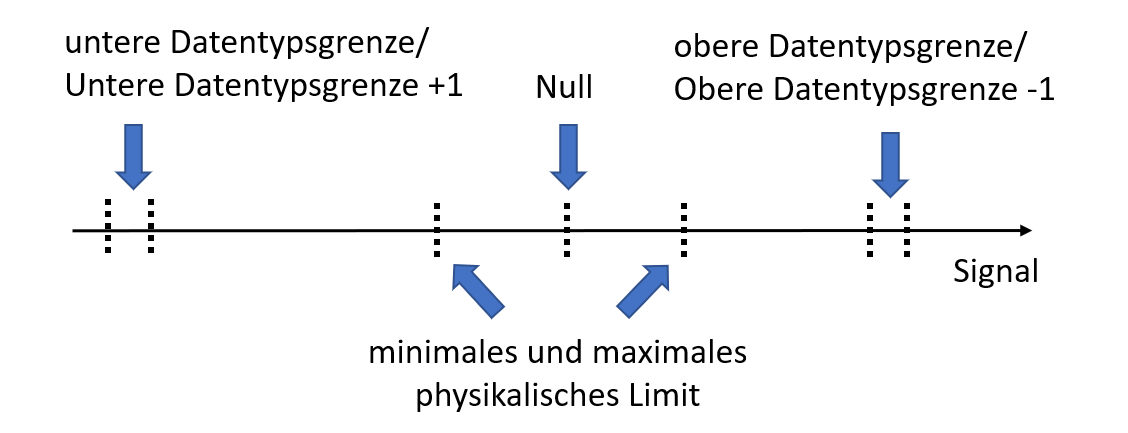
\includegraphics[scale=.9,]{Bilder/EquiZeitstrahl/QuicktestSignalstrahl.png}
\caption{Quicktest Werte auf einem Signalstrahl \cite[vgl.][]{quicktestc}}
\end{figure}
Es werden jeweils die untere und obere Datentypsgrenze als Werte genommen. Das ist im Sinne einer Grenzwertanalyse, denn
Grenzwerte verursachen oft ein fehlerhaftes Verhalten \cite[vgl.][S. 36]{integration}. 
Es wird jeweils eine Ganzzahl unter der oberen und eine Ganzzahl über der unteren Grenze getestet. Die Null wird auch getestet.
Ein physikalisches Limit kommt hier auch vor. Das ist ein Relikt, in dem eine Konvertierung und Skalierung zwischen zeitdiskreten Werten auf den vollen
Datentypsbereich stattfand. Es hat jetzt keine Bedeutung mehr.\par% und muss nicht mehr getestet werden.

In Abbildung 3.3 ist ein Flussdiagramm zu sehen. Es zeigt die Logik eines Schnittstellentests, wie sie in der Quicktest.c 
geschrieben ist. 
Im späteren Verlauf wird der Einfachheit halber ein Ein- und Ausgangssignal gesprochen, die im Folgenden kurz erklärt werden.
\begin{description}
\item[Ausgangssignal] Ein Signal, das aus der ersten Komponente austritt.
\item[Eingangssignal] Ein Signal, das in die zweite Komponente eintritt.
\item[Eine Schnittstelle] verbindet das Ausgangssignal mit dem Eingangssignal.
\end{description}
Zuerst wird das Ausgangssignal auf einen der Werte gesetzt. Es wird die Funktion aufgerufen, in der
die Schnittstelle im Code steht. Daraufhin wird das Eingangssignal überprüft. Der Test ist erfolgreich, wenn 
das Eingangssignal denselben Wert hat wie der Wert, auf die das Ausgangssignal gesetzt wurde. Hat das Eingangssignal einen
anderen Wert, so ist der Test fehlgeschlagen \cite[vgl.][]{quicktestc}\cite[vgl.][]{quicktestlog}.
% Wenn das Eingangssignal auf den Wert ist, der Wenn es den gleichen Wert wie der Wert, der
% dem Ausgangssignal zugewiesen wurde, besitzt, so ist der Test erfolgreich. Wenn es ein anderer Wert ist, so ist der Test fehlgeschlagen.
% %wie eine Schnittstelle durch die Quicktest.c getestet wird.
%Im Nachfolgendem ist ein Flussdiagramm, wie eine Schnittstelle durch die Quicktest.c getestet wird:

\begin{figure}[h]
\centering
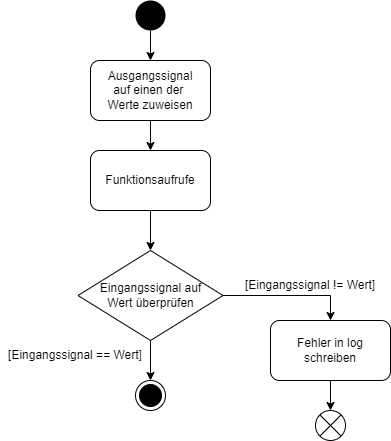
\includegraphics[scale=.6,]{Bilder/Quicktest/QuicktestLogik.drawio.png}
\caption{Quicktest Logik \cite[vgl.][]{quicktestc}}
\end{figure}











% Schnittstellentest:\\ 
	% - Signalverbindungen zwischen der FUs testen:\\
	  % Ausgangssignal einer FU wird zum Eingangssignal der zweiten FU. Test, ob diese Verbindung besteht\\
	% - Testablauf: Ausgangssignal wird auf einen Wert gesetzt und es wird überprüft, ob es als Eingangssignal in der zweiten FU ankommt

% Ein c sharp Skript erzeugt die Datei Quicktest.c\\
% C sharp Skript:\\
% Parsen der xml\_info.xml, darin findet er Out und In Labelverbindungen, sowie Datentyp
% Und Ordner zu .txt Dateien: Funkltionsaufrufe, wo die Verbindung zwischen Ausgangslabel und Eingangslabel hergestellt wird\\

% Quicktest.c wird inklusive des Gesamtprojekts kompiliert und gelinkt\\

% Quicktest.c:\\
% 1. Ausgangslabel einer FU wird auf Werte gesetzt, \\
% 2. Funktionsaufruf, wo die Verbindung der FUs hergestellt wurde\\
% 3. Wert wird am Eingangslabel überprüft\\

% Auf welche Werte gesetzt?\\
% Abhängig vom Datentyp, auf unteren und oberen Grenzwert, 0, physical Min und physical Max 
% Falls float: Fehlertoleranz auf 0.00001f, Überprüfen Eingangslabel auf <  und   > der Fehlertoleranz

% EIN BEISPIEL MIT SDC OUT STB IN IDCFILD ZEIGEN

% Entweder einen Wert oder alle Werte der Schnittstelle

% % Beispiel:
% % m_ACS_Public_ACS_TASKCLASS11.ACS_Out.Umod = (CONV_ONE_FLOAT32)(-3.402E+38);

% % m_PTS_Private_PTS_TASKCLASS11.PTS_In.UmodPhy < (CONV_ONE_FLOAT32)((-3.402E+38) - (0.00001f)) ||
      % % m_PTS_Private_PTS_TASKCLASS11.PTS_In.UmodPhy > (CONV_ONE_FLOAT32)((-3.402E+38) + (0.00001f)) )


% %zweiter Sinn des Quicktests:
% %Überprüfen auf Gleichheit der Datentypen von Ein und Ausgangslabel
% % Überpüfen, ob Signale einer Schnittstelle den gleichen Datentyp haben, typecast der Signale zur Überprüfung

% % Grenzwerte des Datentyps überprüfen, auch mit typecast auf Datentyp
% % 0 Wert überprüfen, ohne typecast

% 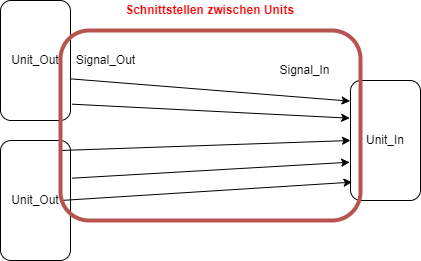
\includegraphics[scale=.6,]{Bilder/Quicktest/AnalyseQuicktest.drawio.png}
% \textbf{Bildinfo Schnittstellen:\\
% Klärung, was eine Schnittstelle ist}
		\newpage
		\section*{Potenziale}
			%\newpage
Ein Potenzial des Quicktests ist, dass die Laufzeit verbessert werden kann. Um die Schnittstellen zu überprüfen, ist es
nicht nötig das Gesamtprojekt zu kompilieren, da jeweils nur eine C Datei einer Komponente benötigt wird. 
Um es möglich zu machen, dass jeweils 
nur eine C Datei pro Komponente analysiert wird, muss die Verbindung zu anderen Dateien getrennt und mit einem Platzhalter ersetzt werden.
Dieses Abtrennen wird auch Stubben genannt \parencite[S. 337]{integration}.
Nach dem Status Quo ist das Stubben nicht möglich, da das Gesamtprojekt zu 
einer \ac{exe} kompiliert wird. Beim Kompilieren zu einer \ac{exe} werden alle Abhängigkeiten benötigt und es kann nicht gestubbt werden.
Mit TPT können Dateien gestubbt werden.

% Das bestehende Konzept hinter dem Quicktest ist, dass das Gesamtprojekt inklusive der Quicktest.c kompiliert und gelinkt wird. 
% Es werden alle Sourcen kompiliert, da der Compiler alle Abhängigkeiten benötigt. Aufgrund der Größe des Projekts dauert das Kompilieren
% länger als eine Stunde.
% %(Die daraus resultierende exe wird ausgeführt und ein log Datei wird beschrieben.)
% Das große Potenzial besteht darin, dass es
% nicht nötig ist, das Gesamtprojekt zu kompilieren, da pro Unit jeweils nur eine einzige Source benötigt wird. Es wird eine 
% Möglichkeit gesucht, dass nur die bestimmten Sourcen auf die Schnittstellen überprüft werden. TPT bietet dafür die Option,
% dass für den Schnittstellentest unbedeutende Dateien gestubbt werden. 

Ein weiteres Potenzial ist, dass ein Ordner mit Artefakten im Projekt hinfällig gemacht werden kann und somit 
auch nicht gepflegt werden muss. Es gibt nämlich einen Ordner, in denen Funktionsaufrufe des Quicktests je Komponente
in Text-Dateien stehen. Indem ein Parser sich für den Quicktest automatisiert die Funktionsaufrufe zusammensucht, 
müssen die Dateien nicht mehr abgelegt werden.
Dadurch erreicht man, dass die Funktionsaufrufe immer up to date sind und nicht mehr händisch gepflegt werden müssen.
% Die Funktionsaufrufe für den Quicktest liegen in
% einem Ordner dauerhaft ab. Vermutlich wurde die Liste einmal manuell erstellt. Dies ist nicht von Vorteil, da bei 
% dementsprechenden Veränderungen auch die Liste mit den Funktionsaufrufen per Hand gepflegt werden müssen. Es wäre
% sinnvoll diese Informationen automatisiert zu bekommen. Damit wären die Funktionsaufrufe immer up to date und es
% wären die Artefakte auch nicht im Projekt abgelegt.








% Gründe, warum Quicktest langsam ist:\\
% Alle Sourcen werden kompiliert\\

% Es wird eine exe erzeugt, die Softcar übergeben wird\\
% Um eine exe zu erhalten müssen ALLE Sourcen kompiliert werden, da Compiler alle Abhängigkeiten(includes etc) benötigt\\


% Einmaliger Funktionsaufruf, um Werte einer FU Task zu übergeben, anstatt für jedes Label einzeln den Funktionsaufruf zu starten\\

% Eine exe wird erzeugt, da Softcar eine exe benötigt. TPT ebnötigt keine exe. TPT kann Fehlende Softwareteile stubben.\\


% Artefakte (Funktionsaufrufe) werden in einem Ordner abgespeichert und dann vom C Sharp Skript benutzt. 
% Das macht man nicht! Es sollten die Infos für die Funktion geparst werden und dann im Skript benutzt. Diese Infos müssen nicht in einem Ordner dauerhaft gespeichert werden
		\chapter{Sourcenmodell für den Quicktest}
			%% \lstdefinestyle{customc}{
  % belowcaptionskip=1\baselineskip,
  % breaklines=true,
  % frame=L,
  % xleftmargin=\parindent,
  % language=C,
  % showstringspaces=false,
  % basicstyle=\footnotesize\ttfamily,
  % keywordstyle=\bfseries\color{green!40!black},
  % commentstyle=\itshape\color{purple!40!black},
  % identifierstyle=\color{blue},
  % stringstyle=\color{orange},
% }
%\lstset{escapechar=@,style=customc}
%\newcommand{\includecode}[2][c]{\lstinputlisting[caption=#2, escapechar=, style=custom#1]{#2}<!---->}
%\includecode{Code/STB_Private_df.h}



% \lstinputlisting[style=customc, caption=TestfallmitDatafield.c]{Code/TestfallmitDatafield.c}
% \lstinputlisting[style=customc, caption=SDC\_Public\_dfi.h]{Code/SDC_Public_dfi.h}
% \lstinputlisting[style=customc, caption=STB\_Private\_dfi.h]{Code/STBPrivatedfi.h}
% \lstinputlisting[style=customc, caption=ZIL\_STB\_dfi.h]{Code/ZIL_STB_dfi.h}
			% Die Software ist komplex und hat viele Abhängigkeiten. Eine Datei alleine ist nicht genug.
% Auch im Hinblick auf TPT. Es ist Stand jetzt immer noch nicht möglich das Gesamtprojekt zu analysieren.
% Eine Komponente, nämlich SCB, kann kompiliert werden. Dahingegen einzelne Dateien innerhalb der Komponente
% können widerum nicht alleine kompiliert werden. Aus diesen Gründen wurde eine C Datei 
% nachgestellt. Diese Datei soll so viele Informationen wie die reale Datei haben, jedoch
% alle Abhängigkeiten, die nicht für den Quicktest gebraucht werden.
% So wenig wie möglich, so viel wie nötig.
% Nach design pattern von ZF werden die Schnittstellen in <Komponentenname>\_Task.c definiert.
% Die Signale sind in Makros versteckt, somit benötigt das Modell eine .c Datei mit allen Makros,
% die die Signale brauchen.
% Die Software hat viele Abhängigkeiten
In diesem Kapitel wird eine C Datei für den Quicktest nachgestellt. Diese wird benutzt, um einen einfachen Schnittstellentest
in \ac{tpt} durchführen zu können. Weiterer Code aus der Datei, der nicht für den Quicktest benötigt wird, wird weggelassen.

In der Datafield stecken Informationen über die Signale und deren Schnittstellen. Um diese Schnittstelleninformationen
im Code zugreifbar zu machen, werden Makros in Header Dateien generiert. Diese Header Dateien werden durch einen include-Guard der C Datei bekannt gegeben (siehe Abbildung 4.1). Damit hat die C Datei Zugriff
auf die Schnittstellen. Die Makros werden im Code verwendet, um die Signale zu verbinden, sodass eine Schnittstelle entsteht.


% Die C Datei, in der die Schnittstelle definiert ist, hat Abhängigkeiten zu anderen Dateien, die jedoch größtenteils nicht für den Quicktest benötigt werden.
% Des Weiteren ist das Aufsetzen des Gesamtprojekts in TPT noch nicht abgeschlossen. Um ein Konzept für den Quicktest in TPT erstellen zu können, ohne dass es an Mühen für die Projekteinrichtung bedarf,
% %die Einrichtung des Softwareprojekts stört,
% wird eine C Datei nachgestellt.
% Nach design pattern von ZF werden die Schnittstellen in <Komponentenname>\_Task.c definiert. Die Wertzuweisung der Signale im Sinne der Schnittstelle sind in Makros definiert. Somit benötigt die Nachstellung eine C Datei mit 3 Makros, die in Header Dateien
% definiert sind und von der C Datei eingebunden werden, so wie hier zu sehen ist:\\
%\newpage
\begin{figure}[h]
\centering
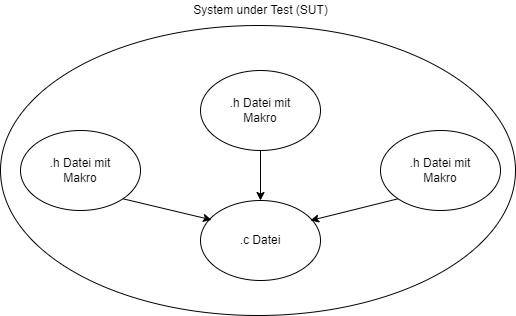
\includegraphics[scale=.6,]{Bilder/Quicktest/Makros.drawio.png}
\caption{Sourcenmodell für den Quicktest}
\end{figure}

% Es wird eine Schnittstelle in der C Datei nachgestellt (siehe Abbildung 4.1). Eine Schnittstelle besteht aus drei Makros.
% %Im Kommentar ist zu sehen, dass es eine einfache Wertzuweisung ist, wenn die Makros aufgelöst sind. 
% Es werden drei Header Dateien mit dem include-Guard eingebunden, in denen Makros stehen.   

In Listing 4.1 ist die C Datei zu sehen. Im Kommentar (Zeilen beginnend mit //) ist zu sehen, 
dass es eine einfache Wertzuweisung ist, wenn die Makros aufgelöst sind.\par
\lstinputlisting[style=customc, caption=C Datei Quicktest]{Code/TestfallmitDatafield.c}
In Listing 4.2 ist eine Header Datei zu sehen. Dieses Makro hat das Prinzip eines Setters. Ein Setter wird in der
objektorientierten Programmierung eingesetzt. Es ist eine Methode, die ein Attribut auf einen Wert setzt. Dieser Wert
wird der Methode als Parameter übergeben. Hier ist es ein Makro und es wird anstatt eines Attributs ein Signal auf einen
Wert gesetzt \parencite[S. 414 f.]{java}.

\lstinputlisting[style=customc, caption=Setter Makro]{Code/STBPrivatedfi.h}
In Listing 4.3 ist die nächste Header Datei zu sehen. Dieses Makro setzt ein weiteres Makro ein.
\lstinputlisting[style=customc, caption=Makro verweist auf ein weiteres Makro]{Code/ZIL_STB_dfi.h}
In Listing 4.4 ist die dritte Header Datei zu sehen. Dieses Makro hat das Prinzip eines Getters und kommt ähnlich
wie der vorher beschriebene Setter aus der objektorientierten Programmierung. Das Getter Makro gibt 
in diesem Fall ein Signal wieder.
\lstinputlisting[style=customc, caption=Getter Makro]{Code/SDC_Public_dfi.h}



Löst man nun alle drei Makros auf, wird wie zuvor schon erwähnt, erkenntlich, dass es eine Wertzuweisung ist. Das Setter Makro bekommt
als Parameter das Getter Makro. Der Wert
des Signals einer anderen Komponente wird in ein Signal dieser Komponente eingesetzt. Dies entspricht einer Schnittstelle.
% Es wird eine Schnittstelle in der C Datei nachgestellt(siehe Abbildung XY). Eine Schnittstelle besteht aus drei Makros.
% Im Kommentar ist zu sehen, dass es einfache Wertzuweisung ist, wenn die Makros aufgelöst sind.
% Es werden drei Header Dateien mit dem include-Guard eingebunden, in denen die Makros stehen.

% %\lstinputlisting{Code/TestfallmitDatafield.c}

% %\lstinputlisting[style=customc, caption=Schnittstelle mit Makros]{Code/TestfallmitDatafield.c}

% In Abbildung XY ist eine Header Datei zu sehen. Dieses Makro hat das Prinzip eines Setters. Eine Setter wird in der 
% objektorientierten Programmierung eingesetzt. Es ist dabei eine Methode, die ein Attribut auf einen Wert setzt. Dieser
% Wert wird der Methode als Parameter übergeben. Der Unterschied zu dem Makro ist: Der Hintergrund ist keine Klasse, sondern
% eine Header Datei. Es ist keine Methode, sondern ein Makro. Es ist kein Attribut, sondern ein Signal\parencite[S.414 f.]{java}.
% Hier ist mehr Text, passt.
% %\lstinputlisting[style=customc, caption=Schnittstelle mit Makros]{Code/STBPrivatedfi.h}
% %\lstinputlisting[style=customc, caption=SetterMakro]{Code/STBPrivatedfi.h}

% % In Abbildung XY ist die nächste Header Datei zu sehen, in dem ein Makro definiert ist.
% % Dieses Makro verweist auf ein weiteres Makro.
% % \lstinputlisting[style=customc, caption=Makro verweist auf weiteres Makro]{Code/ZIL_STB_dfi.h}

% % In Abbildung XY ist die letzte Header Datei zu sehen. Darin ist das Makro definiert, worauf das vorherige Makro verwiesen hat.
% % Dieses Makro hat das Prinzip eines Getters und kommt ähnlich wie der vorher beschriebene Setter aus der objektorientierten
% % Programmierung. Das Getter Makro gibt den Wert eines Signals wieder.
% % Löst man die Makros des Getter und des Setter auf, bekommt man eine Wertzuweisung, wie es im Kommentar in Abbildung XY zu sehen ist.
 % % % eines Signals von einer zweiten Komponente
 % % % auf das andere Signal. Das Getter Makro holt ein Signal von einer Komponente. Das Setter Makro setzt ein Signal der Komponente auf einen Wert.
% % In das Setter Makro wird als Parameter das Getter Makro eingesetzt.
% % Das Getter Makro holt den Wert eines Signals von einer anderen Komponente und dieser Wert wird durch das Setter Makro 
% % auf ein Signal in dieser Komponente gesetzt.
% % \lstinputlisting[style=customc, caption=Getter Makro]{Code/SDC_Public_dfi.h}




% % In dieser Header Datei ist das Makro SDC Public, es zeigt auf ein Signal.(Code zeigen) Getter mit java als Quelle

% % In dieser Header Datei, Makro: in dem Makro ist ist ein weiteres Makro (Header Makro in Makro zeigen)

% % in dieser Header Datei: Makro zeigt auf STB Label. Setter mit java als Quelle

% % Des Weiteren sind die Signale in einer C Datei definiert. Um diese Datei TPT bekannt zu machen, muss im TPT Wrapper diese Datei eingebunden werden.
% % Es gibt schon eine Datei namens vs\_includes intern, die alle structs der Signale einbindet. Diese wird im TPT Wrapper eingebunden.


% % Danach Code zeigen und Getter, Setter erklären.
		


	\chapter{Implementierung des Quicktests in TPT}
		%Schlussfolgerungen aus den Analysen
			%\section{Implementierung des Quicktests in der neuen Toolumgebung TPT}
		In diesem Kapitel wird der Quicktest in \ac{tpt} überführt.
Es werden die Einstellungen in \ac{tpt} getroffen. Es werden die Testfälle erstellt und schließlich wird ein Skript 
geschrieben, das die Testfälle automatisiert generiert.
\section*{C Platform Konfiguration}
\begin{description}
\item[Compiler auswählen] Pfad zu mingw Installation (C Compiler)% /scwcc\_tools/FRD/tools/pc/mingw %installiert zu einem installierten Compiler
\item[Sourcen auswählen] nach design pattern alle <Komponente>\_Task.c %und Einbinden der Datafield C Dateien im Wrapper%Dateien Diese werden später gelinkt und kompiliert, zu analysierende Sourcen müssen auf analysieren gestellt werden
% dabei werden die ausgewählten Sourcen kompiliert und diejenigen, die auf zu analysieren gestellt sind, werden analysiert
% für GSIL: alle \_Task.c auf set analyze setzen
\item[Scheduler] Funktionsaufrufe in Task Dateien
\item[Step size] 125\textmu s
\end{description}
Vom bestehenden Quicktest gibt es einen Ordner,
%(scwcc\_ec\_tc/Integrationstest/Softcar/SIL\_Files/QTestFunctions)
wo pro Komponente die Funktionen, in denen die Schnittstellen definiert sind, aufgeführt sind (siehe Kapitel 3).
%Des Weiteren wird im Wrapper die Datei eingebunden, die die Datafield C Dateien einbindet, in denen die Signale definiert sind.

\section*{Testfallerstellung}
%Die Daten der Schnittstellen können aus der Datafield wie in der Analyse des bestehenden Quicktests entnommen werden.
Die notwendigen Schnittstelleninformation für die Testfallerstellung können aus der Datafield entnommen werden (siehe Kapitel 3).
%Die notwendigen Daten für die Testfallerstellung werden wie in der Analyse des Softcar-Quicktests unter Generieren derQuicktest.c entnommen.
Das physikalische Limit wird nicht vom bestehenden Softcar-Quicktest aufgenommen, da es wie vorher beschrieben ein Relikt ist und nicht mehr benötigt wird.
In \ac{tpt} werden die Testfälle als Step Liste mit folgendem Inhalt erstellt:
\begin{description}
\item[Channel Step] Ausgangssignal auf einen der Werte zuweisen
\item[Compare Step] Eingangssignal mit Wert vergleichen, falls float: mit 0,00001 Fehlertoleranz
\item[wait] @
\end{description}
%Für alle Werte werden nacheinander die Testfälle in die Step Liste geschrieben.
Hier ist ein Beispiel eines Testfalls in der Step Liste:
\begin{figure}[h]
\centering
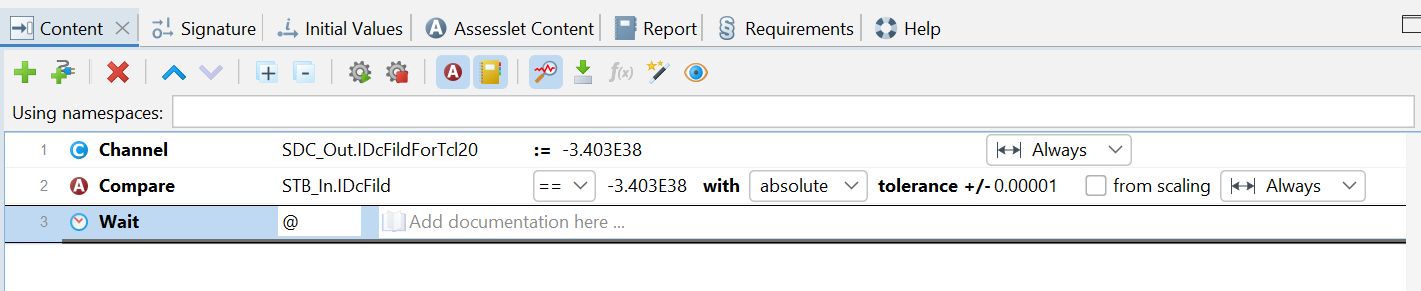
\includegraphics[scale=.6,]{Bilder/Quicktest/Testfallerstellung.png}
\caption{Schnittstellen Testdesign}
\end{figure}
				%\subsection{Testfallerstellung}
					%\input{Abschnitte/Umsetzung/Testfallerstellung.tex}
					%\begin{figure}[!h]
    \centering


  \begin{tikzpicture}%[every node/.style={rectangle,draw,text width=14em,align=center}]
    [
      % Stil für Ein- und Ausgabe
      io/.style={trapezium, trapezium left angle=70, trapezium right angle=110, fill=magenta!10, draw=magenta},
      % Stil für Operationen
      op/.style={rectangle, fill=orange!10, draw=orange},
      op4/.style={rectangle, fill=green!20, draw=green},
			op2/.style={rectangle, fill=green!20, draw=green, minimum height=2cm, minimum width=38mm},
			op3/.style={rectangle, fill=orange!10, draw=orange, minimum height=2cm, minimum width=38mm},
      % Stil für Entscheidungen
      cn/.style={diamond, aspect=2, inner sep=1pt, fill=red!10, draw=red, minimum width=20mm, minimum height=14mm},
      cn2/.style={diamond, aspect=2, inner sep=1pt, fill=blue!20, draw=blue, minimum width=20mm, minimum height=14mm},% Distanz zwischen den Knoten
      node distance=4mm]
    % Knoten
    %\node[op4] (class) {GSIL Projekt als Ausgang};
    
    \node[op4] (init) {C-Plattform Konfiguration};
    \node[op4, below=of init] (list) {Analysieren der Dateien};
    %\node[op, below=of list] (firstitem) {select first item in list};
%    \node[cn2, below=of list] (cond1) {};
    \node[op4, below=of list] (compile) {Generieren des TPT Testrahmens und Kompilieren};
    \node[op4, below=of compile] (depnewlist) {Testfallerstellung};
    \node[op4, below=of depnewlist] (execution) {\textit{Execution} Konfiguration};
    \node[op4, below=of execution] (final) {Testdurchführung};
%    \node[cn2, below=of depnewlist] (cond2) {};
    %\node[op, right=of cond2] (wrongdep) {select next item};
    %\node[op, below=of cond2] (makefiles) {search for item in dictionary to get makefiles};
    % \node[op4, below=of cond2] (initdep) {initialize object using item};
    % \node[op4, below=of initdep] (addobject) {add to object list};
    % \node[cn2, below=of addobject] (cond3) {\shortstack{last item from \\ dependency list?}};
    % \node[op4, right=of cond3] (wrongdep) {select next item};
    % \node[op4, below=of cond3] (findsubs) {object.findSubdirectories()};
    % \node[op4, below=of findsubs] (findfiles) {object.findFiles()};
    % \node[cn2, below=of findfiles] (cond4) {\shortstack{last item from\\ object list?}};
    % \node[op4, left=of cond4] (wrongobject) {select next item};
    % \node[op4, below=of cond4] (end) {Ende};
    
    \path[->]
		%(class) edge (init)
		(init) edge (list)
		(list) edge (compile)
		(compile) edge (depnewlist)
		(depnewlist) edge (execution)
		(execution) edge (final);
      % (finddep) edge (depnewlist)
      % (depnewlist) edge (cond2)
      % (cond2) edge (initdep)
      % (initdep) edge (addobject)
      % (addobject) edge (cond3)
      % (cond3) edge node[above=0.2cm] {No}(wrongdep)
      % (cond3) edge node[right=0.2cm] {Yes} (findsubs)
      % (findsubs) edge (findfiles)
			% (findfiles) edge (cond4)
      % (cond4) edge node[above=0.2cm] {No}(wrongobject)
      % (cond4) edge node[left=0.5cm] {Yes} (end);

    % \draw[->] 
      % (wrongdep) --  ++(2,0) |- (cond2)
      % (wrongobject) -- ++(-2,0) |- (cond1);
		% \draw[->] (cond2) -- node[below] {Nein} ++(2.9,0) -- (entscheid);
		% \draw[->] (cond4) -- node[below] {Nein} ++(4.0,0) -| (gescheitert2);
		% \draw[->] (cond3) -- node[below] {Nein} ++(-4.0,0) -| (gescheitert3);
      %(wrongdep) edge (cond1);
			% (cond1) edge node[right] {Ja} (cond2)
			% (cond2) edge node[below] {Ja} (gesetz2);
    
    % \node[cn, align=center, below=of begehren] (cond1) {okay\\Unterschriften?};
		% \node[cn, align=center, below=of cond1] (cond2) {Landtag nimmt\\Gesetzentwurf an?};
		% \node[op3, align=center, right=of cond1] (gescheitert) {Volksbegehren\\gescheitert};
		% \node[op, align=center, right=of cond2] (entscheid) {Volksentscheid};
		% \node[io, below=of entscheid] (abstimmung) {Stimmen Sie ab!};
		% \node[cn, align=center, below=of abstimmung] (cond3) {Mehrheit stimmt\\mit Ja?};
		% \node[cn, align=center, below=of cond3] (cond4) {Mehr als ein Drittel\\aller Stimmberechtigten\\ stimmt mit Ja?};
		% \node[op2, align=center, below=of cond4] (gesetz) {Gesetz};
		% \node[op3, align=center, right=of gesetz] (gescheitert2) {Volksbegehren\\gescheitert};
		% \node[op3, align=center, left=of gesetz] (gescheitert3) {Volksbegehren\\gescheitert};
		% \node[op2, align=center, left=of cond2] (gesetz2) {Gesetz};
    % % Kanten
    % \path[->]
    %   (begehren) edge (cond1)
		% 	(entscheid) edge (abstimmung)
		% 	(abstimmung) edge (cond3)
    %   (cond3) edge node[right] {Ja} (cond4)
		% 	(cond4) edge node[right] {Ja} (gesetz)
		% 	(cond1) edge node[right] {Ja} (cond2)
		% 	(cond2) edge node[below] {Ja} (gesetz2);

    % \draw[->] (cond1) -- node[below] {Nein} ++(2.8,0) -- (gescheitert);
		% \draw[->] (cond2) -- node[below] {Nein} ++(2.9,0) -- (entscheid);
		% \draw[->] (cond4) -- node[below] {Nein} ++(4.0,0) -| (gescheitert2);
		% \draw[->] (cond3) -- node[below] {Nein} ++(-4.0,0) -| (gescheitert3);

  \end{tikzpicture}
  \caption{Flussdiagramm TPT Einrichtung \parencite[S. 39]{userguide}}
  \end{figure}

%\textbf{Bildinfo Implementierung Quicktest: Überblick, was man in TPT alles für den Quicktest einstellen muss}

% \section*{Testfallerstellung}
% \section*{C Platform Konfiguration}
% Scheduler, TPT Binding, Auswahl der Sourcen, import interface?, Compiler

% großes grünes Flussdiagrammweg	
					%\input{Abschnitte/Umsetzung/UmsetzungQuicktest.tex}
		\section*{Automatisierung der Testfallerstellung}
				Mithilfe der TPTAPI werden die Testfälle automatisch erstellt.
Die Funktionalität wird anhand von Klassendiagrammen, die sich im Anhang befinden, erklärt.
Es gibt drei wesentliche Klassen im Jython Skript, nämlich Types, Interface und InterfacesByUnit, wobei diese
durch eine Aggregation verbunden sind (siehe Abbildung A.1). Eine Aggregation ist eine Ganzes-Teile-Beziehung \parencite[S.61 f.]{integration}.
In allen Klassen kommen Getter und Setter vor, die in Kapitel 4 erklärt werden.

Die Objekte der Klasse Types (siehe Abbildung A.3) enthalten Informationen des Datentyps für die Signale.
Sie besitzt die Attribute für den Namen des Datentyps, untere und obere Wertegrenze und ob
es eine Fließkommazahl ist sowie dazugehörige Getter und Setter Methoden.

% name, max, min und isFloat und als Methoden alle Getter und Setter zu diesen
% Attributen. Max und min sind die obere und untere Wertegrenze eines Datentyps. IsFloat sagt aus, ob es eine
% Fließkommazahl oder eine Ganzzahl ist. 
Die Objekte der Klasse Interface (siehe Abbildung A.4) enthalten Informationen über eine Schnittstelle, sprich das Ausgangssignal sowie das 
Eingangssignal (siehe Kapitel 3) sowie der Datentyp, der durch ein Objekt der Klasse Types eingebunden wird.
Sie besitzt die Attribute für den Namen des Testfalls und der beiden Signale sowie dazugehörige Getter und Setter.
Des Weiteren besitzt sie Methoden zur Erstellen der Step Liste.

Die Objekte der Klasse InterfacesByUnit (siehe Abbildung A.2) enthalten jeweils alle Interface Objekte einer Unit/Komponente.
Sie besitzt die Attribute für den Namen, den Pfad zur C Datei, in der die Schnittstellen definiert sind und
eine Liste, die sich mit Objekten der Klasse Interface füllt, sowie dazugehörige
Getter und Setter.

% Die Klasse Type aggregiert Interface und Interface aggregiert InterfacesByUnit (siehe Abbildung 5.2). Aggregation ist eine
% Ganzes-Teile-Beziehung\parencite[S.61 f.]{integration}. Es wird auch Behälterklasse genannt.(hierfür keine Quelle)
In Abbildung B.1 ist in einem Flussdiagramm zu sehen, wie die Testfälle generiert werden.
Es besteht im Wesentlichen aus zwei Schleifen. Die große Schleife ist dafür zuständig Testfallordner in TPT zu
erstellen. Jeder Ordner ist einer Komponente zugeordnet, wobei die Ordnerstruktur die gleiche ist wie im Softwareprojekt.
Die zweite Schleife ist innerhalb der ersten Schleife. Darin wird für jede Schnittstelle ein Testfall erstellt und mit
Steps gefüllt.
% \begin{figure}[!h]
% \centering
% 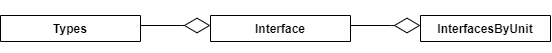
\includegraphics[scale=.8,]{Bilder/Quicktest/Klassen/KlasseAggregation.drawio.png}
% \caption{Aggregation der Klassen}
% \end{figure}
% \begin{figure}[!h]
% \centering
% 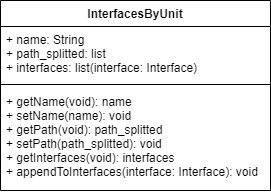
\includegraphics[scale=.9,]{Bilder/Quicktest/Klassen/KlasseInterfacesByUnit.drawio.png}
% \caption{Klasse InterfacesByUnit}
% \end{figure}
% \begin{figure}[!h]
% \centering
% 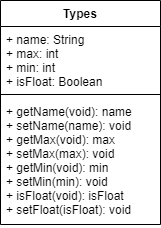
\includegraphics[scale=.9,]{Bilder/Quicktest/Klassen/KlasseType.drawio.png}
% \caption{Klasse Type}
% \end{figure}
% \begin{figure}[!h]
% \centering
% 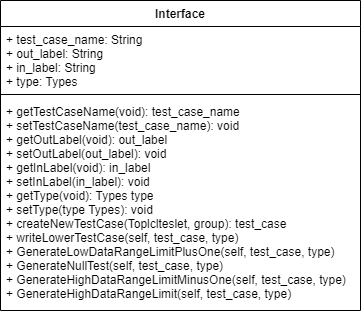
\includegraphics[scale=.9,]{Bilder/Quicktest/Klassen/KlasseInterface.drawio.png}
% \caption{Klasse Interface}
% \end{figure}


% \begin{figure}[!h]
\centering
\begin{tikzpicture}%[every node/.style={rectangle,draw,text width=14em,align=center}]
    [
      % Stil für Ein- und Ausgabe
      io/.style={trapezium, trapezium left angle=70, trapezium right angle=110, fill=magenta!10, draw=magenta},
      % Stil für Operationen
      op/.style={rectangle, fill=orange!10, draw=orange},
      op4/.style={rectangle, fill=green!20, draw=green},
			op2/.style={rectangle, fill=green!20, draw=green, minimum height=2cm, minimum width=38mm},
			op3/.style={rectangle, fill=orange!10, draw=orange, minimum height=2cm, minimum width=38mm},
      % Stil für Entscheidungen
      cn/.style={diamond, aspect=2, inner sep=1pt, fill=red!10, draw=red, minimum width=20mm, minimum height=14mm},
      cn2/.style={diamond, aspect=2, inner sep=1pt, fill=blue!20, draw=blue, minimum width=20mm, minimum height=14mm},% Distanz zwischen den Knoten
      node distance=4mm]
    % Knoten
    \node[op4] (class) {parse xml and fill objects with data};
    \node[op4, below=of class] (list) {select first unit in InterfacesByUnit list};
    %\node[op, below=of list] (firstitem) {select first item in list};
    \node[cn2, below=of list] (cond1) {};
    \node[op4, below=of cond1] (finddep) {create folder if not existing};
    \node[op4, below=of finddep] (depnewlist) {select first interface in interfaces list from unit};
    \node[cn2, below=of depnewlist] (cond2) {};
    %\node[op, right=of cond2] (wrongdep) {select next item};
    %\node[op, below=of cond2] (makefiles) {search for item in dictionary to get makefiles};
    \node[op4, below=of cond2] (initdep) {create new test case};
    \node[op4, below=of initdep] (addobject) {Generate steps according to Test Design using all values};
    \node[cn2, below=of addobject] (cond3) {\shortstack{last interface \\ from unit?}};
    \node[op4, right=of cond3] (wrongdep) {select next interface};
    \node[cn2, below=of cond3] (cond4) {\shortstack{last unit?}};
    \node[op4, left=of cond4] (wrongobject) {select next unit};
    \node[op4, below=of cond4] (end) {end};
    
    \path[->]
      (class) edge (init)
			(init) edge (list)
			(list) edge (cond1)
      (cond1) edge (finddep)
      (finddep) edge (depnewlist)
      (depnewlist) edge (cond2)
      (cond2) edge (initdep)
      (initdep) edge (addobject)
      (addobject) edge (cond3)
      (cond3) edge node[above=0.2cm] {No}(wrongdep)
      (cond3) edge node[right=0.2cm] {Yes} (cond4)
      %(findsubs) edge (findfiles)
			%(findfiles) edge (cond4)
      (cond4) edge node[above=0.2cm] {No}(wrongobject)
      (cond4) edge node[left=0.5cm] {Yes} (end);

    \draw[->] 
      (wrongdep) --  ++(2,0) |- (cond2);
	  \draw[->]
      (wrongobject) -- ++(-2,0) |- (cond1);
  \end{tikzpicture}
    \caption{Automatisierung der Testfallerstellung}
  \end{figure}

% Mit 
% \begin{lstlisting}
    % openResult = TPTAPI.openProject(File("C:\TPTlocal\ProgrammTestfaelle\GenerateTestCases.tptz")) # open tpt-File
    % project = openResult.getProject() # receive the now open project
% \end{lstlisting}
% Wird ein Projekt geöffnet

% topLevelTslt = project.getTopLevelTestlet()
% topLevelTslt.createVariantGroup(nameForGroup, existing\_group)

% Kann man einen Ordner sowie Unterordner erstellen, wo die TestCases stehen

% Mit project.getScenarioOrGroupByName(name)
% Kann man einen TestCase oder Ordner finden


% Mit 
% topLevelTslt.createSLVariant(self.testCaseName, group)
% Kann man einen TestCase erstellen (step list)

% Damit kann man einen step erstellen:
     % test\_case.importTestSpecification("Compare "+self.inLabel+" == "+type.getMin())


% Programmablauf:
% Verbindungsdaten stehen in der xml\_info … hier zeigen wo genau?

% Output eines Skripts erstellt eine xml mit den Daten für mich

	% 1. Xml einlesen
	% 2. Daten in Objekte speichern
	% 3. TPT Projekt konfigurieren, Task.c Dateien zur Analyse setzen
	% 4. Testfälle generieren

% Testfallgenerierung:
% Für jede FU\_Task.c
% Einen neuen Ordner erstellen, wenn noch nicht vorhanden (zB SCB/STB)
% TestCase erstellen
% Testcase mit Steps befüllen
% Ein Testcase ist eine Schnittstelle, getestet nach obere, untere Grenze etc je nach Datentyp

% Durch alle FUs iterieren..
% 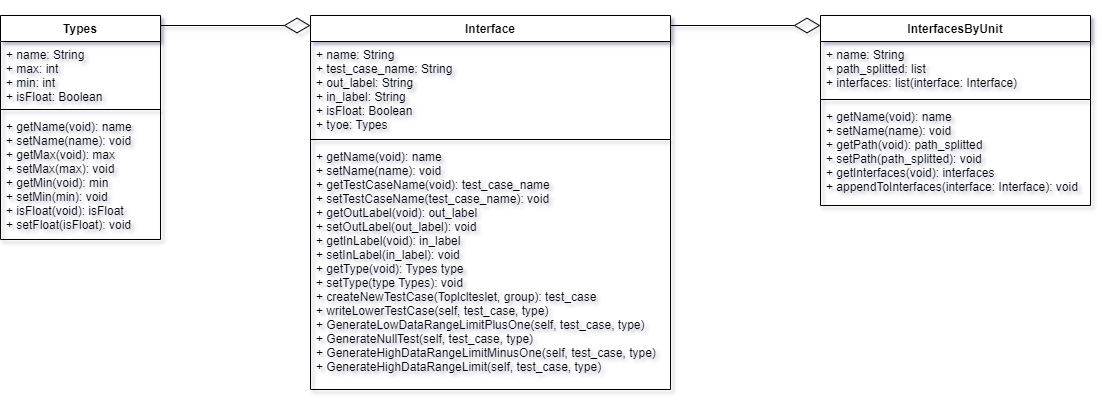
\includegraphics[scale=.3,]{Bilder/Quicktest/QuicktestKlassendiagramm.drawio.png}
% \textbf{Bildinfo Klassendiagramm: die Klassen sind mit Aggregationen verbunden}
% 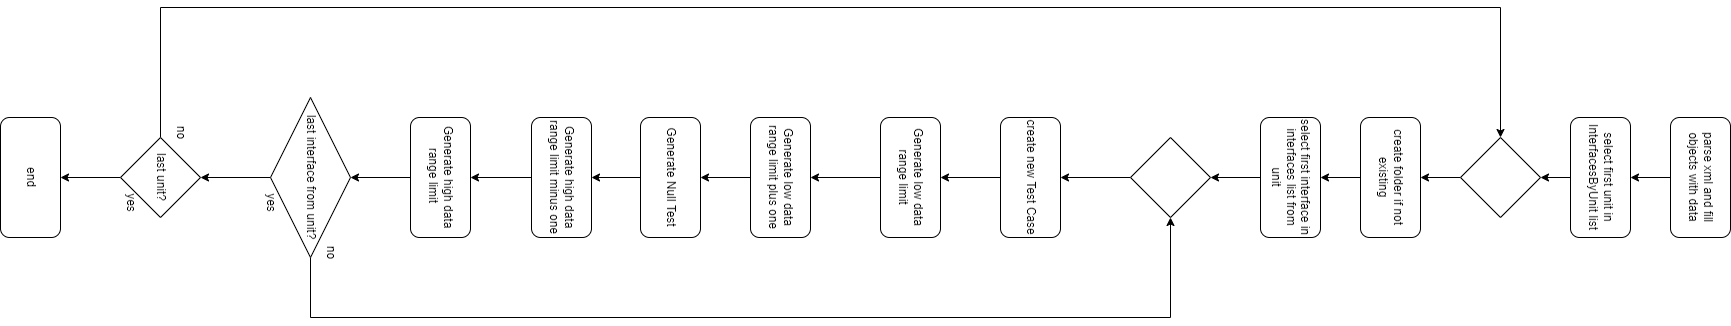
\includegraphics[scale=.4,]{Bilder/Quicktest/QuicktestFlussdiagramm.drawio.png}
% \textbf{Bildinfo Flussdiagramm: Programmablauf vom Generieren der Testfälle}

			%\addvspace{300cm}
	\chapter{Konzept für einen Äquivalenzklassentest in TPT}
		In diesem Kapitel soll ein Konzept erarbeitet werden, wie der Äquivalenzklassentest sinnvoll eingesetzt werden kann.
Es wird gezeigt, wie sie definiert werden können. Es wird eine Selbstüberprüfung gezeigt. 
Es werden bestehende SIL Tests überprüft, ob alle Wertebereiche abgedeckt werden.

Abbildung 6.1 soll als Beispiel einer Berechnung gelten.
% Es wird anhand von folgendem Beispiel in Abbildung 6.1 erklärt.
% Es soll die Berechnung von SDC\_AgAftTiShift getestet werden.
%Es wird als Beispiel SDC\_Current, die Berechnung für SDC\_AgAftTiShift getestet.
%Erklären, wofür diese Größe im Detail da ist.
\begin{figure}[h]
\centering
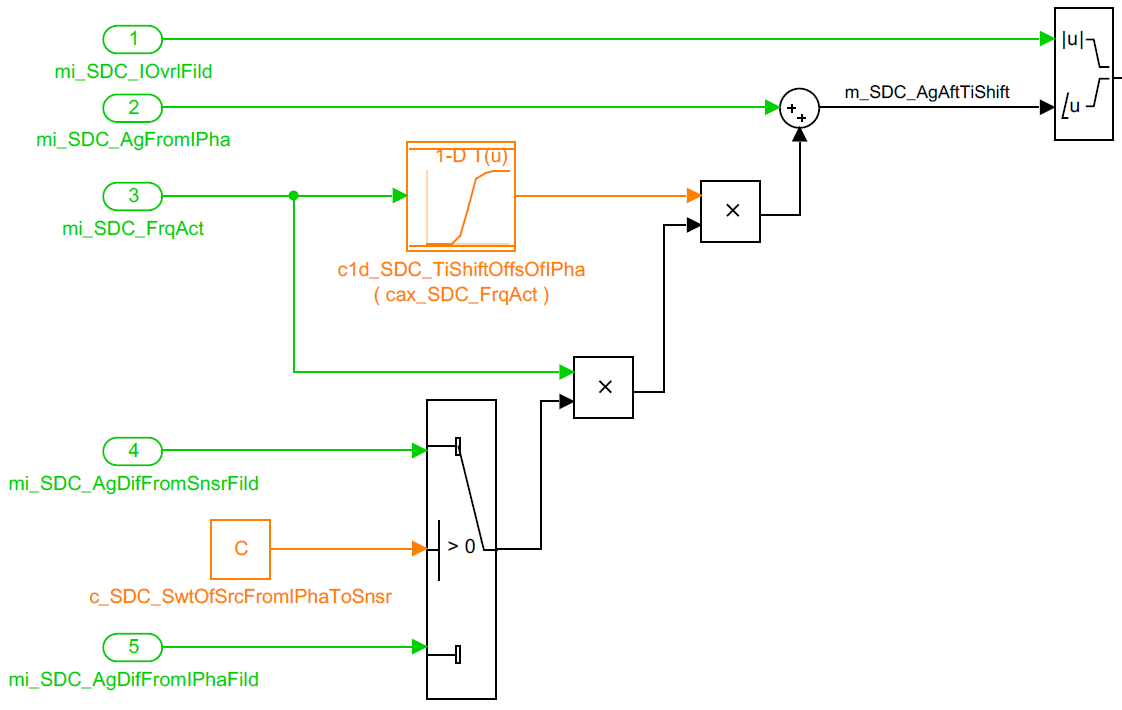
\includegraphics[scale=.9,]{Bilder/SDCDoku.png}
\caption{Beispiel einer Berechnung}
\end{figure}
Es beinhaltet eine Switch, die zwischen zwei Eingangsgrößen umschaltet. Es sind insgesamt
vier mögliche Eingangsgrößen, die durch Addition und Multiplikation sowie einer Funktion ein Ergebnis berechnen.
\section*{Definieren}
Als Grundlage dafür wird ein bestehender SIL Test genommen. Wenn der Test nach dem Requirement 
vollständig und richtig ist, so sind darin alle Werte der Signale enthalten, die für das Requirement notwendig sind.
Diese Werte können als Repräsentanten verwendet werden und dafür ein Wertebereich um den Repräsentanten
festgelegt werden. Eine Äquivalenzklasse soll ein einziges bestimmtes Verhalten abbilden. Dabei sollen alle Werte sich gleich verhalten. 
Wenn es hier Unterschiede gibt, ist es sinnvoll, sie in kleinere Wertebereiche zu zerlegen.
Beispielsweise sollen nach dem Requirement verschiedene Frequenzen getestet werden.
So werden Äquivalenzklassen
für niedrige, für mittlere, eine für hohe und eine für gefährlich hohe Werte erstellt. Es soll zweitrangig sein,
welcher Wert in der jeweiligen Klasse genommen wird, da alle Werte nach dem Requirement gleich anzusehen sind. 
\section*{Selbstüberprüfung}
Mit diesem Test soll überprüft werden, ob sie in sich Sinn machen. Es wird getestet, ob alle Äquivalenzklassen
erreichbar sind. In dem Fall des Beispiels werden alle Wertebereiche der Eingangsgrößen
der Reihe nach gesetzt und es wird überprüft, ob alle Wertebereiche des Ergebnissignals erreicht werden.
Zuerst werden alle Eingangsgrößen auf einen Repräsentanten zur Initialisierung gesetzt.
Eine Step Liste wird nach dem Minimalkriterium mit den gesetzten Äquivalenzklassen durch TPT generiert. 
Bei einer korrekten Definition sollten alle erreicht werden und die Selbstüberprüfung erfolgreich sein.
\section*{Überprüfen bestehender \ac{sil} Tests}
Es werden alle Parameter eines \ac{sil} Tests überprüft.
Dies wird mit dem \textit{Equivalence Class Coverage table} durchgeführt. Der Sinn dieses Tests ist,
den \ac{sil} Test zu validieren. Durch diesen Test wird ersichtlich, ob der \ac{sil} Test bezüglich
der Wertebereiche vollständig ist.
\section*{weitere Einsatzmöglichkeiten}
Um den Äquivalenzklassentest nutzen zu können, müssen zunächst Äquivalenzklassen definiert werden.
Das Definieren ist umfangreich und zeitaufwendig. Es bietet jedoch Vorteile, denn dadurch schafft man eine
Datenbasis an Werten als Repräsentanten beziehungsweise Wertebereichen. Nach dem Status Quo steht der Testfall
im Vordergrund und die Auswahl der Werte für den Test ist nur ein Mittel zum Zweck. Durch die neue Testart 
wird der Blickwinkel auch auf die Testwerte gelegt. Die Auswahl der Werte ist genauso wichtig wie
der Testfall selbst, denn ein Test mit den falsch gewählten Werten ist genauso hinderlich wie ein schlechtes Test Design.
Ein weiterer wichtiger Punkt ist, dass, sobald die Äquivalenzklassen definiert sind, man sie
vielfältig in allen möglichen Testfällen wiederverwenden kann. In TPT ist der Zugriff darauf beispielsweise
in der Step Liste sehr einfach
möglich durch \textit{<Signalname>->ec.random} sowie anderen Schlüsselwörtern (siehe Abschnitt 2.3).
					
					
	\chapter{Diskussion der Ergebnisse}
		\section*{Schnittstellentest}
Es ist nicht gelungen die Laufzeit des Quicktests zu verbessern.
Es ist noch ein großes Potenzial vorhanden, denn TPT muss noch besser für das Softwareprojekt konfiguriert werden.
Derzeit ist es nicht möglich einzelne Dateien von TPT analysieren und kompilieren zu lassen. Da die Schnittstellen
jeweils nur in einer Datei einer Komponente definiert sind, könnte sehr viel Laufzeit eingespart werden.
Das Jython Skript, das die Testfälle für den Quicktest automatisiert generiert, funktioniert soweit. Es legt Ordner an,
so wie es im Softwareprojekt auch der Fall ist, sodass sich Entwickler schnell zurecht finden können.
Es ist zwar nicht die Gesamtlaufzeit verbessert worden, aber es ist jetzt möglich, dass einzelne Komponenten oder gar Schnittstellen alleine getestet
werden.% TPT gibt beim Quicktest einen Fehler aus, Windows Fehler. 
% jeweils nur eine Datei 

% Nicht gelungen den Quicktest zu optimieren(Zeiteffizienz verbessern)
% Testausführung dauert sehr lange, Grund; GSIL hat Probleme in TPT Konfiguration

% Automatisierung der Testfälle, hat gut funktioniert mit TPTAPI
% keinen Parser gebaut, der Funktionsaufrufe für Quicktest findet
% Generell alle Funktionen von den Task.c auf Schedule stellen, beziehungsweise Artefakte Ordner benutzen
% Probleme mit Windows Fehler.. ansonsten funktioniert Quicktest 

\section*{Äquivalenzklassentest}
Es wurde eine gute Grundlage geschaffen, sodass ein Äquivalenzklassentest in naher Zukunft eingeführt werden kann.
Es wurde ein Konzept erarbeitet, das man schnell einführen kann. Es wurde gezeigt, wie \ac{sil} Tests überprüft werden kann. 
Es wurde gezeigt wie Testfälle mit Äquivalenzklassen von TPT generiert werden können. Die große Arbeit ist alle
Äquivalenzklassen für jedes Signal zu definieren. Durch das Definieren wird eine Datenbasis geschaffen, die auch für
andere Tests eingesetzt werden kann. 
% Konzept aufgezeigt, aufgezeigt, dass es machbar ist und auch schnell einsetzbar durch Generieren von
% Äquivalenzklassen 
% schnell einsetzbar, beim Überprüfen der SIl Tests müssen nur alle Signale, die im Test verwendet werden
% als Assesslet Equi angegeben werden plus Definition der Äquivalenzklassen
% Es ist denkbar, ein Skript zu schreiben, das alle Signale, die im Testfall vorkommen, als  Äquivalenzklassen
% Assessment auswählt.
		%Ergebnisse interpretieren, einordnen, Vor und Nachteile 
		
		
	\chapter{Zusammenfassung und Ausblick}
		\section*{Zusammenfassung}
Der bestehende Quicktest von ZF wird analysiert und in TPT übertragen. Es wird ein Code nachgestellt, in der die
Schnittstelle definiert ist.
Es wird ein Skript in Jython
geschrieben, das automatisiert die Testfälle in TPT generiert.

Es wird ein Konzept für den Äquivalenzklassentest vorgestellt. Der Äquivalenzklassentest ist eine gute Erweiterung,
insbesondere für bestehende \ac{sil} Tests. Es wird auch gezeigt, wie Äquivalenzklassen selbst überprüft werden können.
Es wird erklärt, wie Äquivalenzklassen gebildet werden können.
% Durch das Definieren der Äquivalenzklassen wird eine Datenbasis geschaffen, die für weitere Tests in TPT
% eingesetzt werden können. 
% Schnittstellentest, alles gemacht

% Äquivalenzklassentest alles gemacht
% schnell einsetzbar

\section*{Ausblick}
Als Potenzial für den Quicktest wird in Kapitel 3 genannt, dass ein Parser Funktionsaufrufe, in denen die Schnittstellen
definiert sind, finden könnte. Dadurch müssen die Funtionsaufrufe nicht mehr in einem Ordner abgespeichert 
werden. Dieser Parser wurde noch nicht umgesetzt. 
TPT muss weiter für die bestehende Software konfiguriert werden. Wenn es durch die Konfiguration möglich ist, 
dass nur die Dateien, die für den Quicktest nötig sind, kompiliert werden, so ergibt sich auch eine schnellere 
Laufzeit des Quicktests in TPT. Die Äquivalenzklassen müssen für jedes Signal erstellt werden, um Äquivalenzklassentests
einführen zu können.
 % Es ist
% Um den Äquivalenzklassentest einzusetzen, um bestehende SIL Tests zu überprüfen, so 
% Parser der Funktionsaufrufe bauen für Quicktest
% Quicktest Fehler beheben.
% Äquivalenzklassen definieren
% Äquivalenzklassen definieren plus in SIL TPT Assesslets richtig einsetzen(alle Signale in Assesslet von SIL Tests
% angeben)
		% \section{Zusammenfassung}
			% Ziele der Bachelorarbeit erreicht?
			% Gedanken von Einleitung aufgreifen
		% \section{Ausblick}
			% neue offene Fragen (Ausblick)
			% was konnte nicht umgesetzt werden und warum? (Ausblick)
		\label{LastPage}
		\newcounter{letzte}
		\setcounter{letzte}{\value{page}}
		
		
	
			
	\addchap{Eidesstattliche Erklärung}
		\pagenumbering{roman}
		\setcounter{page}{\value{generell}}
		Die vorliegende Abschlussarbeit wurde von mir selbstständig verfasst und nur mit den angegebenen
Quellen und Hilfsmitteln angefertigt. Wörtliche und sinngemäße Zitate im Text sind als solche 
gekennzeichnet.
% Hiermit erkläre ich, dass ich die vorliegende Arbeit selbständig und ohne Benutzung anderer als der angegebenen
% Hilfsmittel angefertigt habe. Alle Stellen, die wörtlich oder sinngemäß aus veröffentlichten und nicht veröffentlichten
% Schriften entnommen sind, sind als solche kenntlich gemacht. Die Arbeit ist in gleicher oder ähnlicher Form - auch auszugsweise -
% noch nicht im Rahmen einer anderen Prüfung vorgelegt worden.

\vspace{70pt}
Schweinfurt, 30. April 2022
\hspace*{\fill}\begin{tabular}{@{}l@{}}\hline
\makebox[6cm]{Xaver Gruber}
\end{tabular}
%\begin{tabular}{@{}l@{}p{3cm}@{}l@{}}\hline
%\makebox[6cm]{Schweinfurt, 30.April 2022} && \makebox[6cm]{Xaver Gruber}
%\end{tabular}
	\listoffigures
	\lstlistoflistings
	\appendix
		\chapter{Klassendiagramme der Quicktestimplementierung}
			\begin{figure}[!h]
\centering
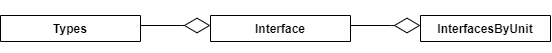
\includegraphics[scale=.8,]{Bilder/Quicktest/Klassen/KlasseAggregation.drawio.png}
\caption{Aggregation der Klassen}
\end{figure}
\begin{figure}[!h]
\centering
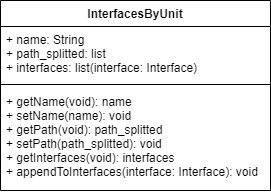
\includegraphics[scale=.9,]{Bilder/Quicktest/Klassen/KlasseInterfacesByUnit.drawio.png}
\caption{Klasse InterfacesByUnit}
\end{figure}
\begin{figure}[!h]
\centering
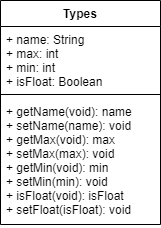
\includegraphics[scale=.9,]{Bilder/Quicktest/Klassen/KlasseType.drawio.png}
\caption{Klasse Type}
\end{figure}
\begin{figure}[!h]
\centering
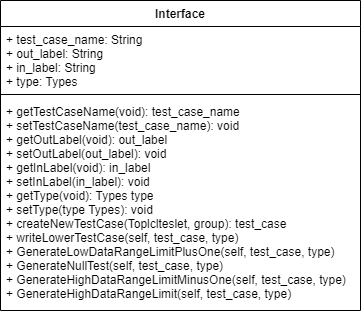
\includegraphics[scale=.9,]{Bilder/Quicktest/Klassen/KlasseInterface.drawio.png}
\caption{Klasse Interface}
\end{figure}
				%\section{Test bla bla}
				% \begin{figure}[!h]
				% \centering
				% 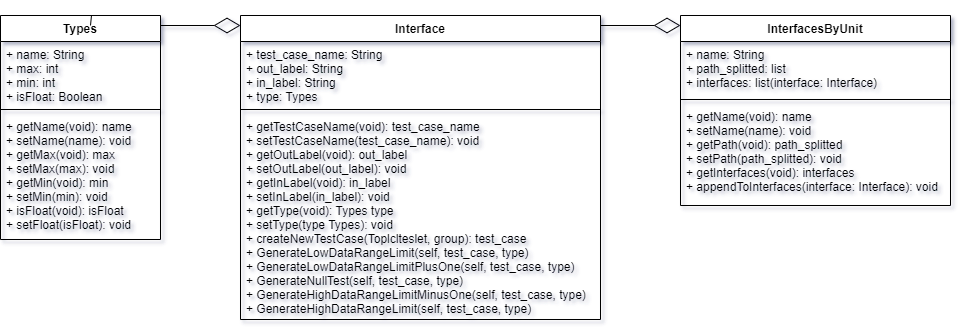
\includegraphics[scale=.5,angle=-90]{Bilder/Quicktest/Klassen/QuicktestKlassendiagramm.drawio.png}
				% \caption{Aggregation der Klassen}
				% \end{figure}
		\chapter{Flussdiagramm der Quicktestimplementierung}
			\begin{figure}[!h]
\centering
\begin{tikzpicture}%[every node/.style={rectangle,draw,text width=14em,align=center}]
    [
      % Stil für Ein- und Ausgabe
      io/.style={trapezium, trapezium left angle=70, trapezium right angle=110, fill=magenta!10, draw=magenta},
      % Stil für Operationen
      op/.style={rectangle, fill=orange!10, draw=orange},
      op4/.style={rectangle, fill=green!20, draw=green},
			op2/.style={rectangle, fill=green!20, draw=green, minimum height=2cm, minimum width=38mm},
			op3/.style={rectangle, fill=orange!10, draw=orange, minimum height=2cm, minimum width=38mm},
      % Stil für Entscheidungen
      cn/.style={diamond, aspect=2, inner sep=1pt, fill=red!10, draw=red, minimum width=20mm, minimum height=14mm},
      cn2/.style={diamond, aspect=2, inner sep=1pt, fill=blue!20, draw=blue, minimum width=20mm, minimum height=14mm},% Distanz zwischen den Knoten
      node distance=4mm]
    % Knoten
    \node[op4] (class) {parse xml and fill objects with data};
    \node[op4, below=of class] (list) {select first unit in InterfacesByUnit list};
    %\node[op, below=of list] (firstitem) {select first item in list};
    \node[cn2, below=of list] (cond1) {};
    \node[op4, below=of cond1] (finddep) {create folder if not existing};
    \node[op4, below=of finddep] (depnewlist) {select first interface in interfaces list from unit};
    \node[cn2, below=of depnewlist] (cond2) {};
    %\node[op, right=of cond2] (wrongdep) {select next item};
    %\node[op, below=of cond2] (makefiles) {search for item in dictionary to get makefiles};
    \node[op4, below=of cond2] (initdep) {create new test case};
    \node[op4, below=of initdep] (addobject) {Generate steps according to Test Design using all values};
    \node[cn2, below=of addobject] (cond3) {\shortstack{last interface \\ from unit?}};
    \node[op4, right=of cond3] (wrongdep) {select next interface};
    \node[cn2, below=of cond3] (cond4) {\shortstack{last unit?}};
    \node[op4, left=of cond4] (wrongobject) {select next unit};
    \node[op4, below=of cond4] (end) {end};
    
    \path[->]
      (class) edge (init)
			(init) edge (list)
			(list) edge (cond1)
      (cond1) edge (finddep)
      (finddep) edge (depnewlist)
      (depnewlist) edge (cond2)
      (cond2) edge (initdep)
      (initdep) edge (addobject)
      (addobject) edge (cond3)
      (cond3) edge node[above=0.2cm] {No}(wrongdep)
      (cond3) edge node[right=0.2cm] {Yes} (cond4)
      %(findsubs) edge (findfiles)
			%(findfiles) edge (cond4)
      (cond4) edge node[above=0.2cm] {No}(wrongobject)
      (cond4) edge node[left=0.5cm] {Yes} (end);

    \draw[->] 
      (wrongdep) --  ++(2,0) |- (cond2);
	  \draw[->]
      (wrongobject) -- ++(-2,0) |- (cond1);
  \end{tikzpicture}
    \caption{Automatisierung der Testfallerstellung}
  \end{figure}
		\chapter{TPTAPI Funktionen}
		%WichtigeTPTAPIFunktionenerklaert.tptapi
			%\lstinputlisting[style=customc, caption=C Datei Quicktest]{Code/TestfallmitDatafield.c}
			\lstinputlisting[style=customc, caption=TPTAPI Funktionen]{Code/WichtigeTPTAPIFunktionenerklaert.tptapi}

	\printbibliography

\end{document}